\thispagestyle{empty}

{\large\fakereceipt{

\noindent\mbox{  } \mbox{  }CELSO FAVARETTO \hspace{0.2cm}\mbox{  }CELSO\\
, \hspace{0.1cm}\mbox{  }A CONTRACULTURA, \hspace*{-0.1cm}\mbox{  }A CON\\
O \mbox{  }ENTRE A CURTIÇÃO \mbox{  }ENTRE\\
L \mbox{  }E O EXPERIMENTAL \mbox{  }E O E

\noindent\mbox{\noindent{}ELSO FAVARETTO \hspace{0.25cm}\mbox{  }CELSO FAV\\}
\mbox{ CONTRACULTURA, \mbox{  }A CONTRAC\\}
\mbox{NTRE A CURTIÇÃO \mbox{  }ENTRE A C\\}
\mbox{ O EXPERIMENTAL \mbox{  }E O EXPER}

\noindent\mbox{\noindent{}ETTO \hspace{0.2cm}\mbox{  }CELSO FAVARETTO \hspace{0.3cm}\mbox{  }C\\}
\mbox{TURA, \mbox{  }A CONTRACULTURA, \mbox{  }A\\}
\mbox{TIÇÃO \mbox{  }ENTRE A CURTIÇÃO \mbox{  }E\\}
\mbox{ENTAL \mbox{  }E O EXPERIMENTAL \mbox{  }E}

\noindent\mbox{\noindent{}TO \mbox{  }\mbox{  }CELSO FAVARETTO \hspace{0.3cm}\mbox{  }CEL\\}
\mbox{RA, \mbox{  }A CONTRACULTURA, \mbox{  }A C\\}
\mbox{ÇÃO \mbox{  }ENTRE A CURTIÇÃO \mbox{  }ENT\\}
\mbox{TAL \mbox{  }E O EXPERIMENTAL \mbox{  }E O}

\noindent\mbox{\noindent{}O \hspace{0.2cm}CELSO FAVARETTO \mbox{  }\mbox{  }CELSO\\}
\mbox{A, A CONTRACULTURA, \mbox{  }A CON\\}
\mbox{O \mbox{  }ENTRE A CURTIÇÃO \mbox{  }ENTRE\\}
\mbox{L \mbox{  }E O EXPERIMENTAL \mbox{  }E O E}

\noindent\mbox{\noindent{}LSO FAVARETTO \hspace{0.2cm}\mbox{  }CELSO FAVA\\}
\mbox{CONTRACULTURA, \mbox{  }A CONTRACU\\}

}}

\pagebreak
\thispagestyle{empty}

\movetooddpage

A partir dos anos 1950,\footnote{Texto
  publicado anteriormente em \textsc{MODOS}: Revista de História da Arte, v.1,
  n.3, 2017.} simultaneamente a grandes transformações
políticas, econômicas, tecnológicas e culturais, a produção artística
respondeu a seu modo aos desafios tecnológicos políticos e ideológicos
que tensionavam o país, compondo projetos de renovação artística e
cultural voltados à efetivação da modernidade. Até o final dos anos
1960, as diversas tendências experimentais haviam transformado a
paisagem da arte brasileira, tanto em termos formais como em relação a
posicionamentos ético"-estéticos. Com a promulgação do Ato Institucional
n° 5, em 13 de dezembro de 1968, o processo artístico"-cultural, tal como
vinha se desenvolvendo nas últimas décadas, foi em grande parte
inviabilizado; a vigorosa atividade que tensionava as relações entre
experimentalismo e política, vanguarda e participação, foi interrompida
com o recrudescimento da censura, com as prisões e o exílio, forçado ou
não, de muitos artistas.

A passagem da década de 1960 para a de 1970 foi marcada por esse
acontecimento -- um duro golpe sobre os projetos e ações políticas e
artístico"-culturais, sobre verdades e ilusões que mobilizaram o desejo e
o empenho de transformação social, às vezes compondo atitudes radicais
de resistência. Sob este ponto de vista, a década de 1970 abriu"-se sob o
signo de uma grande derrota. A expressão ``vazio cultural'' foi aplicada
naquele momento por uma certa vertente crítica exatamente para indicar a
impossibilidade de continuidade ou a inadequação daqueles projetos de
transformação. Contudo, a expressão, que se tornou corrente, só dava
conta de um lado do que acontecia -- a interrupção do extraordinário
trabalho coletivo de comprometimento com os imperativos da justiça e da
liberdade --, sem dar a devida atenção a algo diverso também voltado
para o mesmo interesse -- uma passagem da crítica social e política do
tema aos procedimentos, pondo em destaque as virtudes da invenção; uma
mudança na representação política, advinda inclusive em decorrência do
balanço crítico que começava a ser feito dos ideais, das estratégias e
das ilusões políticas claras ou implícitas nos processos artísticos e
culturais do período que findava.

Assim, é preciso assinalar o outro lado da questão: desde o momento
tropicalista surgiam manifestações culturais diferenciadas,
alternativas, que se estenderam aos anos 1970. Contracultura,
marginalidade, curtição e desbunde foram designações que pretendiam dar
conta de uma produção variada e dispersa, embora constituindo uma trama
feita de alguns tópicos comuns -- que se distinguia daquelas da maioria
dos projetos anteriores, principalmente pela ênfase agora atribuída aos
aspectos comportamentais, à emergência do corpo como espaço de
agenciamento das atividades, aparentemente sem conotação política, desde
que o modo como até então se fazia a arte política fosse tomado como
modelo. A proposição de uma ``nova sensibilidade'', que se compunha com
uma certa concepção de ``marginalidade'' em relação ao sistema
sócio"-político e artístico"-cultural, aparecia como a motivação básica
daquelas manifestações -- o que implicava mudança acentuada da ideia e
das práticas de participação desenvolvidas na década de 1960. Nova
sensibilidade e marginalidade articularam"-se frequentemente ao
experimentalismo nas atividades artísticas e na atividade crítica. É da
intersecção desses conceitos operacionais,\footnote{Cf. Silviano
  Santiago, `` Abutres: a literatura do lixo''. \emph{Revista Vozes.}
  ano 66, v. \textsc{LXVI}, n. 10. Petrópolis: Vozes, 1972, p.~21. Rep. em
  \emph{Uma literatura nos trópicos.} São Paulo: Perspectiva, 1978
  (Debates"-155).} identificadores das manifestações alternativas em
geral, que surgiram as mais expressivas produções culturais da primeira
metade dos anos 1970, que, aliás, não deixavam de se opor à ditadura do
regime militar, portanto de afirmarem um outro modo do político.

Esta atividade multifacetada, convivia com o fato de que o sistema da
arte estava em pleno desenvolvimento, em consonância com o expressivo
incremento da indústria cultural -- em parte articulada às iniciativas
da política oficial, que, por meio de um programa de ação cultural e da
proposição de uma política nacional de cultura, centradas na perspectiva
de modernização conservadora, visava tanto a um relacionamento com os
meios artísticos e intelectuais como ao aproveitamento das novas
possibilidades técnicas para a efetivação das ideias de cultura nacional
e identidade cultural. Várias análises empreendidas sobre a produção
cultural dos anos 1970 destacaram prioritariamente as questões
referentes à consolidação de um mercado de bens simbólicos e aquelas
referentes à concepção oficial de política cultural e seus
desdobramentos institucionais.\footnote{Sérgio Miceli (org.).
  \emph{Estado e cultura no Brasil.} São Paulo: Difel, 1984; Renato
  Ortiz. \emph{A moderna tradição brasileira.} São Paulo: Brasiliense,
  1988.} Uma parte significativa das análises da produção artística do
período situou"-se no horizonte destas questões, ora tematizando as
transformações provocadas pela crescente importância dos meios de
comunicação de massa, ora os impactos da censura e da repressão do
regime militar sobre a produção artístico"-cultural, ora as repercussões
no trabalho universitário das direções teórico"-críticas provenientes do
estruturalismo francês e suas consequências em vários setores,
especialmente no jornalismo cultural e na crítica de arte.

Respondendo às novas condições da sociedade, especialmente ao
alinhamento do país à lógica cultural da sociedade de consumo, a
complexa e variada produção artística, agora inclui, sem preconceitos,
como elemento constitutivo de experimentações, de teorizações e da
crítica, os pressupostos, as regras e as técnicas da indústria cultural.
Institucionalização da cultura, consumo e experimentação, especialmente
quando pensados -- nas artes plásticas, por exemplo -- em relação a
obras ou manifestações efêmeras, conceituais e comportamentais,
evidenciaram problemas ético"-estéticos -- além dos simplesmente
técnicos, de realização, de distribuição ou exibição -- que questionaram
a tentativa de constituição de um sistema da arte, especialmente de um
emergente mercado, que logo se mostraria inconsistente. Ao mesmo tempo,
tal composição iria discutir a viabilidade, a eficácia crítica e o poder
de resistência de toda a produção que se queria alternativa.

Portanto, foi ao lado das iniciativas culturais oficiais, mobilizadoras
de um conjunto de agências, Instituto Nacional do Cinema, Embrafilme,
Funarte, Pró"-Memória, etc., ao lado dos desenvolvimentos de um mercado
de arte e de manifestações variadas não articuladas diretamente às
direções acima, que se desenvolveram as manifestações culturais
alternativas, particularmente as contraculturais, da curtição, ou
desbunde. Na verdade, estas designações recobriam uma gama muito
elástica de manifestações culturais, artísticas e comportamentais;
modalidades e formas diversas de produção alternativa, nas artes, no
jornalismo, nos movimentos sociais. Importa, assim, ressaltar a produção
de artistas e pensadores que geraram um espaço de reinvenção situando"-se
nas margens ou à margem do sistema artístico e social -- sempre em busca
de um fora da negociação com as instâncias estabelecidas --, em parte
desenvolvendo e especificando atividades culturais e experimentações que
vinham das décadas anteriores, seja tentando ressignificar as ações
políticas seja explorando as possibilidades técnicas dos novos meios e
linguagens, às vezes novamente tentando articular transformações das
linguagens e resistência política.

A produção artístico"-cultural dos 1970, longe de um suposto vazio,
instaurou um processo extensivo de invenção, que incluía a reelaboração
das experiências anteriores, à margem da política oficial de cultura e
da indústria cultural. As manifestações de cultura alternativa,
particularmente a direção contracultural, configuraram, entre o final da
década de 1960 e meados da de 1970, uma atitude e ações de grande
vitalidade, em que se percebia uma descrença em relação ao alcance
revolucionário da arte propugnado na década anterior, afirmando outras
formas de modos de assimilação e mesmo de militância política.

\asterisc

O estado da cultura brasileira no início dos anos 1970, com destaque
para as experiências contraculturais, precisa ser esclarecido, para que
se possa considerar que o período não foi o do vazio cultural, mas cheio
de outras significações culturais, artísticas e políticas de fronteira,
interessadas em novas formas de subjetividade. Entre 1971 e 1974, a
revista \emph{Visão,} através de entrevistas com intelectuais e artistas
relevantes, detectou sintomas de uma ``crise da cultura brasileira'' e,
a partir daí, fez em números sucessivos um diagnóstico dos ``impasses da
cultura'', tanto investigando as razões da crise como possíveis saídas
do que entendia como ``vazio cultural ``que vinha tomando conta do
país'' desde a edição do \versal{AI}"-5 e o incremento da censura.\footnote{``A
  crise da cultura brasileira'', \emph{Visão}, 05/07/1971, p.~52.} Na
primeira matéria, de 5 de julho de 1971, apareceu a expressão vazio
cultural -- que, como foi informado posteriormente,\footnote{Elio
  Gaspari; Heloisa Buarque de Hollanda; Zuenir Ventura. \emph{Cultura em
  trânsito: da repressão à abertura.} Rio de Janeiro: Aeroplano, 2000.
  Neste livro foram coligidos artigos dos autores no período 1971-1986.}
foi cunhada por Zuenir Ventura -- em contraposição aos sucessos na
economia, assim entendia os ``impasses da cultura'' :

\begin{quote}
o desaparecimento da temática, da polêmica e da controvérsia na cultura,
a evasão dos nossos melhores cérebros, o êxodo de artistas, o expurgo
nas universidades, a queda na venda dos jornais, livros e revistas, a
mediocrização da televisão, a emergência de falsos valores estéticos, a
hegemonia de uma cultura de massa buscando apenas o consumo
fácil.\footnote{\emph{Visão}, 05/07/1971, p.~52.}
\end{quote}

É interessante comparar este diagnóstico de dois outros: um de 1º de
março de 1967 que, na efervescência artística e política, identificando
aquela imbricação de ênfase experimental e participação política, do que
acontecia no teatro, na música popular, no cinema, nas artes visuais e
na literatura o diagnóstico assim via em grandes linhas o percurso da
arte brasileira nos anos 1960:

\begin{quote}
Logo depois de 1964, a primeira reação da arte brasileira foi rebelar"-se
e constatar uma situação que a deixara perplexa; em seguida foi
reformular o processo de conscientização e de análise da nova realidade;
e a terceira foi violentar, destruir, chegar ao zero para tentar então
reconstruir.\footnote{``As marcas da inocência perdida''. \emph{Visão},
  01/03/1967, p.~46.}
\end{quote}

Nesta trajetória eram destacadas as ambiguidades e contradições das
posições de artistas e dos projetos artístico"-culturais que se
construíam tendo em vista a retomada da pesquisa inaugurada pelo
modernismo de 22 de ``descoberta do Brasil'', colocando em debate a
contradição entre uma ``tentativa de volta às origens, no momento em que
a internacionalização se torna cada vez mais uma contingência econômica,
sociológica e política inexorável'' e a desmistificação dessa posição
nas atividades artísticas, na ``arte suja'' que se fazia na ocasião. Na
edição de 24 de março do mesmo mês, a matéria ``A cultura posta em
questão'', a partir de um documento oficial -- o ``Diagnóstico
Preliminar da Cultura'' -- e ouvindo artistas e produtores musicais,
discutia as ``condições extraordinárias'' do governo Costa e Silva
``para realizar um programa de alto alcance nacional'', que a partir do
diagnóstico, considerava ``que a atividade cultural deve sair do estágio
espontâneo em que se encontra, no caso de um país
subdesenvolvido''.\footnote{``A cultura posta em questão''.
  \emph{Visão,} 24/03/1967, p.~47.} O diagnóstico, ao propor uma visão
otimista do estado de cada área artística, das bibliotecas, televisão e
editoras, era contraposto nesta matéria às dificuldades colocadas pela
censura, em contradição com o pretendido avanço cultural comandado pelo
governo. Mas a resposta das artes foi outra, como se sabe. De fato, das
proposições do \versal{CPC} da \versal{UNE}, como emblemática de um modo de radicalização
do social e do político nas artes, até as atividades irreverentes dos
tropicalistas do final da década, todas, em sua diversidade e mesmo em
desacordo, manifestavam uma unidade de ação sintomática, contra os
cálculos do regime e, particularmente contra a censura e repressão
política e social.

Só para se ter uma ideia do que é preciso pensar quanto às variadas
estratégias que provinham da intersecção do estético com o político no
final dos anos 60, alvo imediato da repressão do regime com a edição do
\versal{AI}"-5, basta relembrar produções mais significativas que apareceram no
incrível ano de 1967 -- que se estenderam no ano seguinte e que deram
origem a outras nas diversas direções. O filme \emph{Terra em}
\emph{transe}, de Glauber Rocha; a encenação de \emph{O Rei da Vela}
pelo Teatro Oficina de José Celso; e de \emph{Arena conta Tiradentes} no
Teatro de Arena de Augusto Boal; o tropicalismo do grupo baiano; a
exposição \emph{Nova objetividade brasileira}, onde aparece
\emph{Tropicália}, a emblemática manifestação ambiental de Hélio
Oiticica; os livros \emph{Panamérica}, de José Agrippino de Paula,
\emph{Quarup}, de Antonio Callado e \emph{Pessach: a travessia}, de
Carlos Heitor Cony. \textbf{Nestas obras} os signos da complexa situação
cultural -- em que referências das culturas populares, inovações das
práticas artísticas de vanguarda, cada vez mais assimilados pelos
processos da indústria cultural em franco desenvolvimento -- articulavam
projetos e ações culturais de resistência às iniciativas da política
cultural do regime militar.

Assim, entende"-se que a proposição do vazio cultural fundou"-se na
suposição de ausência nos anos 1970 do fervor criativo e da crítica
social ao modo do que aqueles tempos evidenciavam. Entende"-se também,
porque devido à potência crítico"-criativa daquele período, e a
expectativa de retomada do mesmo impulso, ainda que dificultada pela
censura, não se apontava no diagnóstico de Zuenir Ventura, a
possibilidade de a contracultura ser também considerada uma das
variáveis das tentativas de superação dos impasses apontados, certamente
porque suas proposições não se coadunavam com o que se esperava como
enfrentamento do suposto vazio. De fato, a revista \emph{Visão,}
continuando a discussão sobre os impasses da cultura, na importante
matéria de 11 de março de 1974, com o título ``Da ilusão do poder a uma
nova esperança'' (p.~137-155), abria"-se com uma incisiva proposição:

\begin{quote}
Ao contrário da economia e tanto quanto a política, a cultura brasileira
viveu nesses dez anos alguns de seus momentos mais dramáticos e
sofridos. Caminhando da onipotência à impotência, do choque à apatia,
dividida entre os apelos fáceis do conformismo e o seu compromisso
crítico, a criação intelectual atraiu ódios e suspeitas, e mergulhou no
vazio e na fossa. Agora, amadurecida pelo sofrimento, busca de novo a
vontade, abre"-se ao diálogo e alimenta"-se de uma esperança: a de que a
liberdade tantas vezes invocada lhe seja restituída: não como um favor
concedido, mas como direito adquirido, como atributo natural do
pensamento.
\end{quote}

Em suas quatro seções, `` A perda da ilusão'', ``A perda da inocência'',
``A perda da vontade'' e ``A volta do querer'', a rememoração da derrota
de 1964 com a perda das apostas no poder transformador da arte; em
seguida a reconstrução a partir de 1965 das formas de participação e de
protesto pelo exercício das ousadias experimentais que aliavam crítica
política e crítica moral com a proposição de uma arte"-ação
transgressiva, chocante e violenta; depois do \versal{AI}"-5, o desânimo pela
cessação dessa atividade cheia de paixão toda feita de rupturas
artísticas, ``indícios esparsos'' estariam sugerindo, ou possibilitando
o vislumbre, de ``sensíveis modificações de atitude'', fruto de um
processo de auto"-análise da cultura que estava produzindo aos poucos o
abandona da lamentação das derrotas e a autopiedade quanto às
contingências das tentativas de reação à violência e violentações da
ditadura, especialmente crítica das estratégias amparadas em equívocos
na análise da situação. Mas nenhuma menção se fazia, nesses ``indícios
esparsos'', da atividade contracultural que tomava impulso desde 1969.

Mas o próprio Zuenir Ventura, no artigo ``A falta de ar'' de agosto de
1973, ao considerar que o vazio cultural era na verdade um ``vazio
cheio'', pela primeira vez cita a contracultura como uma manifestação
cultural ativa no período. Ao perguntar sobre do quê estaria sendo
preenchido o vazio, distingue as seguintes vertentes culturais: ``uma
cultura de massa digestiva, comercial, de simples entretenimento'';
``uma contracultura buscando nos subterrêneos do consumo, mas
frequentemente sendo absorvida por este, formas novas de expressão e
sobrevivência''; uma cultura explicitamente crítica, tentando olhar a
realidade política e social imediata''.\footnote{Elio Gaspari et. al
  (orgs.). op. cit. p.~59-60.} Apesar das ressalvas, pode"-se
acentuar que o artigo indica uma percepção de aspectos fundamentais da
experiência contracultural: é ``subterrânea'' (que é a designação mais
apropriada, segundo Hélio Oiticica, a essa cultura da divergência);
indica ``formas novas de expressão'' (com que se pode entender as
singulares manifestações artísticas dos novos modos da experimentação
deslocados pela ênfase nos comportamentos) e ``novas formas de
sobrevivência'' (que indica a aposta dos protagonistas da contracultura
na eficácia da nova sensibilidade, dos novos comportamentos, dos novos
valores, opostos e resistentes aos da vida burguesa e da sociedade
industrial).

\asterisc

Fenômeno híbrido e complexo, em parte confluindo e sendo expressão local
do \emph{underground} norte"-americano, estas manifestações
contraculturais eram ambivalentes, oscilavam entre comportamentos
neo"-românticos, e outros que articulavam uma nova sensibilidade
contracultural ao experimentalismo artístico dos anos 1950/1960. Essas
vertentes foram abertas pelas experiências radicais que configuraram um
``momento tropicalista'' da cultura brasileira, emblematizado
basicamente na atividade tropicalista dos músicos baianos, na do Oficina
e outras manifestações correlatas, na antiarte ambiental de Hélio
Oiticica. Poesia, música, cinema, teatro, artes plásticas, literatura,
jornais, revistas, livros, compunham uma produção dispersa e
multifacetada, que não deixava de ser a seu modo uma contestação ao
Brasil do milagre econômico. Pode"-se falar, assim, genericamente, de um
pós"-tropicalismo, sem que a expressão guarde relação imediata com o
pós"-modernismo que aos poucos se irradiava em consonância com a
afirmação em toda parte da lógica cultural do capitalismo avançado.
Pertencente a uma direção mais ampla de cultura e resistência à
ditadura, a ``cultura alternativa'', que se expandiu durante toda a
década de 1970 abrigando tanto manifestações associadas ao
\emph{underground} como a de jornais e revistas, como \emph{Opinião,
Movimento}, \emph{Ex,} esse pós"-tropicalismo, identifica aqui um tipo de
produção artística aliada a posições culturais e comportamentos que
privilegiavam as ``vivências'', a vida cotidiana, a arte fora dos
registros consagrados, enfim, a tudo que poderia ser considerado
marginal à cultura estabelecida, da antiarte de Hélio Oiticica, das
proposições artístico"-terapêuticas de Lygia Clark, de produções
informadas pela poesia concreta, pela onda do conceitualismo, da arte
pobre e da arte do corpo.\footnote{Cf. nota introdutória de \emph{Arte
  em Revista} -- 5. São Paulo: Kairós/\textsc{CEAC}, 1981, p.~3-4.}

Portanto, trata"-se de pensar a especificidade da experiência
contracultural no horizonte mais amplo da cultura alternativa.
Precisamente: em quais produções artísticas pode"-se flagrar modos de
articulação do experimentalismo dos anos 1960, especialmente aquele do
tropicalismo, aos rituais da nova sensibilidade contracultural, às
condições novas do circuito de arte, ao jogo com o mercado e,
finalmente, a uma certa significação política que se diferencia daquela
dos anos 1960.

Importa, assim, discutir a interpretação sobre essa produção,
particularmente a contracultural, feita por Luciano Martins em 1979, e
que ficou consagrada, no ensaio ``A Geração \versal{AI}"-5'', em que reiterando a
ideia de ``vazio cultural'', entendeu que aquela contracultura teria se
manifestado em agrupamentos da juventude oriundos de segmentos das
classes médias dos grandes centros urbanos, por um comportamento de
caráter reativo, alienante e a"-político, de oposição ao autoritarismo
político e à crise familia``A proposição geral deste ensaio é a de que
tais valores, práticas e comportamentos, que são vividos como
contraculturais, acabaram por se transformar, em virtude dos equívocos
sobre os quais se assentavam, num anti"-projeto de liberação; mais:
constituem uma expressão da alienação produzida pelo próprio
autoritarismo e, ao mesmo tempo, são também instrumentos de
alienação''.\footnote{Luciano Martins. ``A geração \textsc{AI}"-5 (Um ensaio
  sobre autoritarismo e alienação''. \emph{Ensaios de Opinião -- 11.}
  Rio de Janeiro: Paz e Terra, set. 1979, p.~74} Para ele, três fenômenos
expressariam, pela construção de tipos ideais, que compareceriam,
isolados ou em intersecção, com frequência e intensidade diversas em
contextos e experiências diversas, a sua caracterização da
contracultura: o uso das drogas, a desarticulação do discurso e o
modismo da psicanálise.\footnote{Luciano Martins. ``A geração \textsc{AI}"-5 (Um
  ensaio sobre autoritarismo e alienação''. \emph{Ensaios de Opinião --
  11.} Rio de Janeiro: Paz e Terra, set. 1979, p.~74} Tais fenômenos
negariam a noção de sujeito em favor da ``exacerbação da
subjetividade'', sem atacar os valores propugnados pelas práticas
autoritárias. Ao reiterar as possibilidades de que o uso das drogas,
transformado em ``culto da droga'', não ter servido efetivamente para
fins de ``liberação pessoal'' com a ampliação da percepção e de
``rebeldia social'', antes tenha desembocado seja em práticas de
``evasão da realidade'' e, até de ``autodestruição'', com que se dava
``denegação tanto da liberdade quanto da condição de sujeito'', o
sociólogo enfatiza que a contracultura teria ficado, a despeito de sua
intenção libertária, refém dos ``sentimentos de vazio e de impotência'',
servindo indiretamente a fins autoritários. Por sua vez, a
desarticulação do discurso, contribuiu para que a atitude significada
por termos como ``curtição'', ``barato'', ``cara'' etc., seriam
indicações da síndrome alienante ``por revelar"-se incapaz de usar a
linguagem e de articular minimamente o pensamento'', atingindo
drasticamente as capacidades de expressão e cognitiva; uma espécie de
afasia em tudo negadora de uma ``visão de mundo'', impossibilitando um
posicionamento existencial e político antiautoritário. E o ``modismo
psicanalítico'' é identificado elemento da síndrome alienante porque a
``expansão da psicanálise'', que efetivamente ocorria naquele momento,
teria decaído em práticas terapêuticas dela dereivadas, como terapia de
apoio, terapia corporal, terapia de grupo etc., que também mais
contribuíram à ``compulsão'' de subjetivação do que na formação de um
sujeito consciente, ativante do processo de resistência aos
autoritarismos, que supostamente estariam sendo criticados.

Sem dúvida, o autor aponta um dos lados da ambivalência constitutiva dos
fenômenos tomados como tipos ideais de sua crítica da contracultura, não
atribuindo valor ao que na experiência contracultural funcionava como
princípios operacionais de uma nova posição, social, política, cultural
e artística. Assim, em sua análise, nenhum indício ou sintoma de vontade
de uma nova atitude referido por Zuenir Ventura estariam presentes na
contracultura -- pelo fato de as ``pautas de comportamento que
caracterizam esse universo se esgotarem ao nível da experiência quase
inarticulada de seus atores; uma experiência meramente instintiva e que
parece destituída de qualquer capacidade de reflexão sobre si própria
enquanto experiência existencial''. Além disso, diz ele, ``o que se
apresenta como contracultura não chegou (ou não chegou ainda) a ser
captado por nenhuma obra"-testemunho -- na literatura, no cinema ou no
teatro -- que seja digna desse nome; quer dizer: de uma obra capaz de
cristalizar o fenômeno e, ao mesmo tempo, a transcender seus aspectos
imediatos através da captação de seu conjunto de
significações''.\footnote{Op.cit. p.~76.}

As expectativas e esperanças na chave do que pensava Zuenir Ventura
podem ser relativizadas e também pode"-se fazer algumas ressalvas à
posição crítica de Luciano Martins -- apesar da importância da sua
análise para a compreensão dos impasses políticos, sociais e artísticos
daqueles tempos. Particularmente, as ressalvas se dirigem ao tipo de
análise que propõe em termos de caracterização da modalidade específica
da experiência contracultural e das categorias artísticas que propõe
para a análise das ``obras'' contraculturais. Pode"-se ressaltar que em
sua especificidade a experiência contracultural foi um fenômeno que não
pode ser simplesmente caracterizado como reativo ou como uma ``síndrome
alienante'', sem relevância para os dispositivos de abertura da cultura
brasileira em vista da reconquista das liberdades subtraídas pelo regime
autoritário. Foi, como aliás assinala Luciano Martins, entre outras
coisas, ``um primeiro instrumento de contestação de um regime (ou de uma
ordem social) percebidos como violadores de um valor
essencial''.\footnote{Op. cit. p.~73-74.} E nem situar as suas ``obras''
no horizonte de expectativas da produção artística institucionalizada
pelo sistema da arte e pelo mercado.

Assim, a questão da contracultura precisa ser pensada através de outros
vetores, sem que se desprezem os citados como atuantes na formulação das
experiências contraculturais. É preciso entender o que significava no
período ``marginalidade'', distinta do que era o alternativo e,
principalmente, entender na atividade artística, a origem cultural da
direção imperante das artes daquele tempo, interessadas, de um lado, na
desestetização como efeito do deslocamento da obra ao comportamento,
inclusive com manifestações típicas de estetização dos comportamentos;
de outro lado, a abertura experimental das artes que podiam ou não
incluir a ênfase no comportamento, mas ativaram forças desatadas pelas
experimentações dos anos 1965-1968.

\asterisc

É possível detectar antes do tropicalismo, a partir de 1964, vários
sintomas de uma atitude contracultural em que esta designação é
associada a manifestações que, genericamente, se opunham à chamada vida
burguesa e às expressões artísticas vigentes, distanciando"-se da relação
imediata entre arte e vida cotidiana e configurando um estilo poético de
vida. Pode"-se destacar, em São Paulo, movimento de ``catequese
poética'', inventado e liderado por Lindolf Bell, de que participavam,
Álvaro Alves de Faria, Carlos Vogt, Luis Roberto Benatti e outros; assim
como os poetas, de extração rimbaudiana e surrealista que apresentavam
marcas da \emph{beat generation,} como Roberto Piva, Claudio Willer,
Antonio Fernando de Franceschi e Roberto Bicelli. No Rio de Janeiro,
Hélio Oiticica, Lygia Clark e Lygia Pape e outros, logo depois da
eclosão do neoconcretismo, colocavam claramente as ideias de vivência e
participação no centro de suas proposições. Oiticica, particularmente,
além disso articulava essas ideias à de marginalidade, desde a invenção
do parangolé, fundante de uma concepção de antiarte, experimental à
margem do sistema da arte. Nestes exemplos, e certamente em outros que
poderiam ser rastreados em vários lugares, observa"-se que outras
experiências de contestação genérica ao sistema da vida burguesa e
particularmente de oposição ao regime militar, diversas das
manifestações críticas situadas no campo hegemônico de esquerda, tão bem
radiografadas no ensaio de Roberto Schwarz ``Cultura e política,
1964-1969'',\footnote{Roberto Schwarz. \emph{O pai de família e outros
  estudos.} Rio de Janeiro: Paz e Terra, 1978.} podem ser assimiladas a
uma larga atitude contracultural.

Mas convém esclarecer que a denominação contracultura, assumiu uma
especificidade nos rastros do tropicalismo, associada às designações de
uma nova atitude caracterizada pela designações ``nova consciência'',
``nova sensibilidade'', ``curtição'' e ``desbunde'', em que a ênfase
recaía no comportamental, na vida aberta, livre do racionalismo, do
autoritarismo, do moralismo e da burocratização. Esta configuração
estava referenciada à produção e atitude dos artistas -- na música
popular, no teatro, nas artes plásticas, na poesia e no cinema.
Particularmente, esta configuração tem como exemplar a produção do grupo
baiano que detonou esta atitude desde o seu aparecimento em 1967,
atitude esta espetacularizada nos aparecimentos na tv, nos shows,
reportagens em jornais e revistas, declarações. Mas, de modo mais
consistente, a atitude aparece na própria estrutura de algumas canções;
por exemplo em ``Alegria alegria'' de Caetano Veloso (``sem lenço sem
documento/ nada no bolso e nas mãos/ eu vou/ por que não?'') ; ``Panis
et circenses'' de Caetano e Gil (``mas as pessoas na sala de jantar/ são
ocupadas em nascer e morrer''); ``Divino maravilhoso'' de Caetano
(``tudo é perigoso/ tudo é divino maravilhoso''). Mais explicitamente a
canção de Gil, de 1969, quando confinado com Caetano na Bahia antes de
partirem para o exílio londrino, de onde retornam em 1972, ``Cultura e
civilização'' (``a cultura a civilização/ elas que se danem ou não''),
além de outras do mesmo disco (``Futurível'', ``Objeto semi"-identificado'') são indicativas de variados signos de uma certa atitude
contracultural, que marcada pelo \emph{underground} norte"-americano e
pelas repercussões do maio de 1968 francês (claramente identificável em
``É proibido proibir'' de Caetano Veloso).

O que ficou conhecido como contracultura, ``nova consciência'' ou ``nova
sensibilidade'', mantinha claras referências ao \emph{underground
internacional em} que a atitude \emph{drop out}, o \emph{cair fora da
sociedade, era veiculado} por meio de revistas, jornais, na músicas e
rituais que pretendiam divulgar princípios de uma nova imagem da vida,
que induzisse a novos comportamentos. Enquanto as maneiras,
neorromânticas, com que apareciam identificava os integrantes dessa onda
contracultural como alienados, quando não, vagabundos, isto é, como
desintegrados dos modos de vida habituais, os comportamentos, na
verdade, portavam inconformismo e desprezo, não simplesmente reativos,
face ao autoritarismo, burocratização e racionalismo da vida social
burguesa. A vida em comunidades, as práticas alimentares naturais, o uso
das drogas, as novas formas de relacionamento afetivo e sexual, o
desprezo pelas fórmulas políticas, pela organização familiar e pela
educação formal, caracterizariam esta outra mentalidade, planetária e
descentralizada, aparentemente desligada da ``cultura e da
civilização'', rumo a uma outra sociabilidade.

O efeito dessa atitude e das novas formas de vida seria subterrâneo,
acreditando na potência dos gestos e comportamentos, menos no debate
explícito de ideias, e desinteressadas das experimentações estéticas. Em
busca de uma nova ética pessoal, a imaginação volta a ser a rainha das
faculdades: dela partiriam os sinais de renovação da vida e da arte,
implicadas em uma expressão marginal, calma, suave e bela de
transformação individual e social. Toda possibilidade de transformação
social proviria da expressão individual medrada nas comunas, nos
encontros coletivos, na comunhão despreconcebida dos corpos, associados
aos ritmos vitais da natureza; daí a articulação de muitas ações de
resistência às intervenções tecnológicas no meio ambiente.

Percebe"-se facilmente como esta compreensão afirmativa da contracultura
pretende"-se livre de contradições e ambiguidades, visíveis pela atitude
distanciada já no período de sua vigência. Pois, a marginalidade era
puramente circunstancial e foi logo integrada pela indústria do consumo.
As condutas os modos de vestir, a linguagem específica, os rituais
teatralizantes, as novas práticas alimentares, o ecologismo, as práticas
corporais e místicas orientais, foram rapidamente recuperados como
produtos diversificados da sociedade do espetáculo. O mercado
enriqueceu"-se de uma variedade nova de objetos exclusivamente destinados
aos jovens, contribuindo para reforçar o mito que nascia: a juventude
prolongada, para todos, que diluía a crença fundada no conflito de
gerações, aludindo ao nascimento de uma cultura pan"-totêmica diluída na
liturgia neo"-totêmica dos objetos. Mas não se pode subestimar a
importância da experiência contracultural para as mudanças de
comportamento, para o alerta quanto à destruição do meio ambiente, para
o processo de relativização da moral dos comportamentos, para a
singularização das vivências na sociedade do controle.

\asterisc

A intersecção entre a nova sensibilidade contracultural, a curtição, e o
experimentalismo tropicalista detonou uma outra orientação na produção
artística e cultural, significativa em termos de ressonâncias para a
abertura da contemporaneidade: um pós"-tropicalismo em que proposições e
obras configuraram emblemáticas intervenções que aliaram
experimentalismo, novos comportamentos e um outro deslocamento da
questão do político na arte e na cultura. Esta produção da primeira
metade dos anos 1970 aliou o gosto pela experimentação, a sofisticação
técnica, o jogo com o mercado, efetivado na segunda metade dos anos 1960
às experiência da curtição, enfatizadoras da gestualidade, do corpo, do
sensorial, das experiências de limite via drogas, misticismo e
comportamentos renovados na vida amorosa, da nova sensibilidade
contracultural. É então na confluência dessas linhas, interessadas ambas
na efetivação de articulações da arte com a vida, que emerge uma arte e
uma crítica da cultura, proveniente da transformação do que restou dos
ensaios de descentralização da cultura propugnada pelo tropicalismo, dos
impasses técnicos e ideológicos da arte de vanguarda em sua relação com
as possibilidades do sistema, e a absorção do comportamental da
contracultura.

Desta discussão e prática participaram artistas novos e artistas
provenientes da década anterior e outros já consagrados. Arnaldo Jabor
publicou no \emph{Pasquim,} no início de 1972, um sintomático artigo em
que, para compreender a intervenção da contracultura na reorganização da
cultura, retraça o percurso da arte e da cultura no Brasil desde o
Modernismo, destacando a importância do ``trauma de dezembro de 68''
para a compreensão dos impasses e indeterminações daquele
momento.\footnote{Arnaldo Jabor. ``Debaixo da terra''. \emph{O Pasquim,}
  no. 131. Rio de Janeiro: Codecri, 10/01/72.} Avaliando o período
1969/1972 e tentando captar a originalidade das experiências
contraculturais, constata que estas, apesar de domesticadas, não
chegaram ao fim como apenas uma grande ilusão:

\begin{quote}
Ficaram os despojos vivos, uma infinita massa colorida, de gestos,
costumes, formas de pensar, de amar, de ver o mundo, que estão para
sempre assimiladas às consciências das jovens gerações. A Cultura morre
nos museus, mas se eterniza dentro do corpo. Jimi Hendrix antes de
morrer disse numa entrevista ao \emph{Rolling Stone} que o negócio já
não era mais aquele que era outro, que ele não sabia qual era, mas que
vinha aí. John Lennon declarou, numa tremenda \emph{ego"-trip} que o
sonho tinha acabado. E continua vivo, e que enquanto há vida haverá
sonho. E para sonhar basta não ter medo da imaginação.
\end{quote}

Também sintomático é o texto \emph{Escrevivendo} de Jomard Muniz de
Britto -- poeta e crítico pernambucano, participante das experiências
educacionais de Paulo Freire na década de 1960 e das discussões sobre
cultura popular, e associado às proposições do tropicalismo e da
contracultura --, publicado em 1973 em edição marginal.\footnote{Jomard
  Muniz de Britto. \emph{Escrevivendo.} Recife: Mimeo, 1973.} Propõe o
conceito de ``desculturação'' como sugestivo da conjugação entre
experimentalismo de vanguarda e a nova sensibilidade, entre vanguarda e
a desculturação:

\begin{quote}
Desculturação é uma proposta na medida em que \qb{}funciona\\
como um estimulante conceitual operacional, palavra\\
de um agir concreto, nome\versal{AÇÃO} de uma realidade como\\
fato e projeto. Não como palavra jogada no vazio. Não\\
como séria metáfora da vacuidade. Quem fala \qb{}descultur\versal{AÇÃO}\\
pensa em des"-condicionamento dos estereótipos da cultura\\
como tabu, em maiúsculo e com K. Da Kultura proibitiva,\\
centralizadora, hierárquica: K\\
(\ldots{})\\
A vanguarda existe por uma d i f e r e n ç a \qb{}diferenci\versal{AÇÃO}.\\
Diferença entre o nível de produção cultural \qb{}(crítico"-criativo,\\
inovador, experimental, laboratorial, inventivo) e o \qb{}horizonte\\
largoestreito do consumo pelo grande público (passivo, \qb{}redundante,\\
repetitivo, enquadrado dentro dos padrões vigentes.
\end{quote}

Esta diferenciação deveria conjugar a racionalidade (exatidão, rigor,
lucidez, estruturação) e a transracionalidade -- abertura para todas as
fontes de experiência humana (magia, mito, misticismo, filosofias). É a
busca de uma totalização, feita na vida pela conjugação de ciência,
filosofia, religião etc. A pergunta que, segundo ele, se colocaria diria
respeito à criticidade e autocriticidade da vanguarda para ser
eficiente, criativa e instauradora. A condição complementar é que a
vanguarda se tornasse verdadeiramente produção, o que a levaria a ser um
trabalho inscrito no corpo pela imaginação corporificada. Utilizando"-se
de formulação de Umberto Eco, diz que a vanguarda se tornaria, assim,
integrada, contra qualquer apocalipse. Como se vê esta teorização,
pretendendo"-se crítica e original, rearticulava as discussões de
vanguarda, tensionadas agora pela concepção de arte"-vida proveniente do
tropicalismo e da contracultura.

Apesar do interesse dessas duas posições, enquanto sintomáticas e
exemplares, é preciso levar em conta trabalhos de artistas que
configuraram a potência da produção artística e da nova crítica cultural
surgida daquele imbricamento de experimentalismo e comportamentos
contraculturais: alguns atuantes nos anos 1960, como Hélio Oiticica,
Lygia Clark, Caetano Veloso, Gilberto Gil, Torquato Neto; outros recém
aparecidos, como Waly Salomão, Rogério Duarte, Torquato Neto, José
Agrippino de Paula, Gramiro de Matos, José Vicente, Antonio Bivar, Júlio
Bressane, Andrea Tonacci, Rogério Duarte, Macalé, Walter Franco. E a
lista poderia ser estendida. Além disso, é preciso ressaltar a
importância das revistas e jornais que difundiram essa produção,
diversificada, com acento, ou no experimental, ou na curtição, ou entre
os dois, como \emph{Navilouca, Polem, Código, Poesia em Greve, Artéria,
Corpo Extranho.}

\asterisc

A nova consciência contracultural teve em Luiz Carlos Maciel o seu guru,
cujas matérias divulgando a nova sensibilidade começaram a aparecer em
1970 no jornal \emph{O Pasquim,} fundado em 1969; incialmente na seção
``Underground'', depois, em encarte, no jornal \emph{Flor do Mal.}
Nestas publicações -- e em outras, como \emph{Verbo, Presença, Rolling
Stone, O Bondinho} -- irradia"-se por Maciel e muitas outras pessoas, uma
visão de vida neorromântica, a figuração de um novo universo cultural,
de uma outra imagem da vida, dos comportamentos, dos valores.

\begin{quote}
Seguinte: o futuro já começou. Não se pode julgá"-lo com as leis do
passado. A nova cultura é o começo da nova civilização. E a nova
sensibilidade é o começo da nova cultura. Sua continuação é a nova
lógica. Não: as leis do passado não servem.

Não se deixe perder pelos demônios cansados da velha Razão. Ela ainda
não conhece o poder dos sentidos da mesma maneira que, durante séculos,
insistiu em ignorar o poder dos instintos. Não se deixe perder. (\ldots{}) Os
limites da velha razão engendra a \emph{nova} sensibilidade.(\ldots{}). A
revolução cultural está em marcha, dizem uns e outros. É verdade. Até em
seus recuos, ela não apenas propõe a mudança: ela muda, aqui e agora,
através de uma dialética que ninguém definiu. Seu método é a vigência
provisória da moda. Através do efêmero ela finca suas raízes. Seu estilo
é o improviso incoerente do músico \emph{free jazz.} Não: ela não deseja
destruir tudo para começar de novo. Prefere assumir sua tarefa montada
sobre os ombros da tradição, sem compromisso, colhendo dessa tradição
suas forças desprezadas: o êxtase, o sonho, o ritmo, a cor, o riso, a
paz e todos os presentes que o nosso Deus criador oferece aos sentidos
humanos para a sua fugaz fruição nesta Terra.\footnote{Luiz Carlos
  Maciel, ``Um manifesto''. \emph{Nova consciência.} Rio de Janeiro:
  Eldorado, 1973, p.~46-48.}
\end{quote}

Nota"-se neste manifesto o eixo da nova sensibilidade ser interpretado
como regressivo, pelo menos se se tiver em mente o modo como tal
sensibilidade tinha operado no tropicalismo, em que as força do êxtase,
o sonho, a beleza, o efêmero, a paz, a moda tinham servido, como na
interpretação do surrealismo feita por Walter Benjamin, para alimentar o
desejo de ruptura, de uma revolução profana, contra o que impedia o
movimento de liberação, na vida, na cultura e na política.\footnote{Walter
  Benjamin, ``O surrealismo -- o mais recente instantâneo da
  inteligência europeia''. trad. Erwin Theodoro Rosental. São Paulo:
  Abril Cultural, 1975 (Col. Os Pensadores), p.~64.} À maneira das
manifestações na Califórnia e em Paris, o surrealismo foi sempre alegado
como referência das insurreições. A crença na mudança da consciência e
dos comportamentos, enfim a aposta na eficácia dos gestos exemplares,
seriam o fundamento de uma atitude política em tudo diversa da
institucionalizada.

É possível perceber o alcance daquelas posições aparentemente tão
descomprometidas, mas afirmativas em suas aparições nas manifestações,
nos modos de vida, nas páginas dos jornais e revistas da curtição: é que
funcionavam pelas derivas, aposta na potência do acontecimento, no
alargamento da racionalidade, por uma modalidade de pensamento que
derivava também do sensível, enfim, operações desterritorializantes.
Além disso, foi o primeiro momento no Brasil em que, como atitude
contracultural, a política de minorias encontrou espaço de afirmação,
com assunção das mulheres, dos negros, dos homossexuais, das práticas
religiosas e corporais resistentes ao dualismo ocidental: orientalismos,
candomblé, umbanda, quimbanda. Particularmente importante foi a
penetração cultural do ideário e práticas contraculturais no que tange
ao cultivo das práticas culturais de raízes orientais e o
desenvolvimento de uma grande variedade de práticas terapêuticas,
corporais, de grupo -- no momento, aliás, em que a psicanálise de
linhagem freudiana, em sua diversidade, e a psicologia analítica de Jung
se difundiam no país.

Pode"-se dizer que a atitude contracultural, à semelhança daquelas
surrealistas e dadá, em muito implica uma estetização da vida. Todas as
manifestações articulavam categorias estéticas modernas que informavam
os comportamentos na vida em comunidades ou nos aparecimentos públicos
(que adquiriam uma certa espetacularidade) e mobilizavam procedimentos
artísticos. O primado do efêmero e do contingente, o desligamento da
ideia de obra de arte, uma arte corporal, comportamental, ambiental; a
recusa do esteticismo modernista, frequentemente em favor do artesanal e
do ludismo como oposição à instrumentalização moderna. Para isto, tanto
na oralidade como na escrita literária e informativa, uma linguagem,
particular, às vezes como um idioleto, foi"-se elaborando nas vivências e
atividades contraculturais, uma linguagem em que a produção da
significação se materializou em experiências inventivas renovadoras da
linguagem literária habitual. O mesmo se deu nas invenções que atingiram
as formas então correntes no teatro, no cinema, nos quadrinhos, na
diagramação de livros, jornais e revistas independentes que, aliás,
foram logo recuperadas pela indústria da cultura.

É exatamente a confluência das repercussões dessa larga atitude
contracultural com a experimentação de artistas -- que vinham caminhando
na direção das mudanças no exercício das artes implicadas na abertura ou
na morte da obra de arte, na assimilação da vida cotidiana na arte e
vice"-versa, como é o caso emblemático de Hélio Oiticica e Lygia Clark --
que gerou uma variada produção em literatura, teatro, cinema,
performances, instalações etc., configurando uma nova expressão
artística, marcada pela ambivalência, em que o político não está
ausente, embora deslocado.

\asterisc

Silviano Santiago, em 1972, em ensaio pioneiro dedicado especificamente
à literatura tensionada pela contracultura e pelo experimental, delineou
argutamente as linhas de força, os antecedentes e os sintomas dessa
produção de que resultou uma espécie de estética da curtição:

\begin{quote}
A curtição (sen"-si"-bi"-li"-da"-de de uma geração, sensação, estado de
espírito, conceito operacional, arma hermenêutica, termômetro,
barômetro, divisor de águas etc.) já foi consagrada pela música popular,
principalmente pelo chamado grupo baiano liderado bifrontalmente por
Caetano e Gil, que comporta grandes realizações, entre elas o
extraordinário primeiro disco dos Novos Baianos. Teve seus momentos de
visualização com os filmes de Rogério de Almeida, Júlio Bressane e
Neville de Almeida, e com as peças de Antônio Bivar e José Vicente.
Criou redações de jornal e de revistas no Rio, em São Paulo e Salvador;
nas bancas \emph{Presença, Bondinho, Rolling Stone, Verbo} etc. A
curtição ocasionou cisões homéricas e irrecuperáveis entre a patota do
\emph{Pasquim} e os seguidores do guri Luiz Carlos Maciel; entre o
pessoal que gosta dos baianos"-que"-voltam e os que são fãs de Milton
Nascimento que"-fica e gosta da sua caipirinha; entre os
bem"-situados"-badalados do cinema novo e os arrivistas malditos do cinema
boca"-do"-lixo, para ficar com alguns exemplos recentes. A curtição
deslocou o eixo da criação da terra"-das"-palmeiras para a London, London,
descentrando uma cultura cuja maior validez e originalidade tinha sido a
de delimitar cultural, artística e literariamente determinada área
geográfica que por coincidência se chamava Brasil. Deslocou o eixo
linguístico luso"-brasileiro para uma espécie de esperanto nova geração,
cristalizado em palavras poucas que se tornam senhas entre os iniciados.
Finalmente deslocou o eixo musical samba para uma certa
latinoamericanidade: todos os ritmos são bons, como disseram Torquato
Neto e Capinam em momento anterior e tropicalista. A curtição foi capa
da revista \emph{Veja} e seguramte assunto da revista \emph{Manchete.} A
curtição é vendida discretamente pelas agências de publicidade (entre na
sua!) através de cartazes na parede, radinhos de pilha e televisão na
sala.\footnote{Silviano Santiago. ``Abutres: a literatura do lixo''.
  Revista \emph{Vozes,} ano 66, v. \textsc{LXVI}, n. 10, 1972, p.~21-22.}
\end{quote}

Nota"-se neste fragmento que o autor refere"-se a expressões artísticas
que resultam do imbricamento dos processos das vanguardas da década
anterior e da assimilação da chamada nova sensibilidade; entretanto,
consciente embora dos impasses daquelas vanguardas, é despida do
heroísmo e do cinismo com que elas pretendiam dar conta das aporias
constitutivas das polarizações ou intercessões entre experimentalismo,
participação política e mercado. Sem a presunção de se aliar a projetos
de ruptura social, consciente de que ao artista não é mais permitida a
ilusão de usar a arte como instrumento de transformação da realidade,
esta arte afirma"-se como lúdica e estranha, como que aderente à
proposição de Hélio Oiticica: só existe o grande mundo da
invenção.\footnote{Hélio Oiticica. Entrevista a Ivan Cardoso.
  \emph{Folha de S. Paulo Ilustrada,} 16/11/85, p.~48; rep. em
  \emph{Encontros/Hélio Oiticica.} org. César Oiticica Filho e Ingrid
  Vieira. Rio de Janeiro: Beco do Azougue, 2009, p.~227.} Então, se de
um lado essa produção dirige"-se a um público específico ativado pelas
experiências contraculturais, de outro, o seu compromisso exclusivo é
com o experimental, que dificulta a legibilidade das obras. Assim, a
nova sensibilidade é assumida como conceito operacional que mobiliza a
invenção de experiências de transmutação da relação entre arte e
realidade -- com que se configura um outro modo do político, centrado
nas mudanças de comportamento interpessoais e comunitários, e não mais
nos projetos totalizadores de mudança social. Entende"-se então que a
nova sensibilidade, enquanto conceito operacional, redimensiona
novamente a posição social da produção artística, provoca antagonismo
entre a nova produção e o público relacionado ao sistema da arte. A
ideia de criação é reinventada, reativada pelas vivências como a única
maneira de se posicionar face à resistência do sistema que mantém a
ordem constituída em termos transcendentes ou pela razão instrumental.

Quer se fale de artes plásticas, literatura, poesia, cinema, teatro ou
música, essa arte que se pretende independente implica uma estética
caracterizada por algumas regras básicas. Em primeiro lugar a
valorização do fragmento em detrimento do todo. Como diz Silviano
Santiago, ``o trecho aparece trabalhado, bordado, rendado, pedindo
portanto apreensão sintética (fragmento) e ao mesmo tempo analítica
(bordado)'',\footnote{Silviano Santiago. id. ibid.} com que se perde a
continuidade, a discursividade, típicas da lógica da exclusão. O
estranhamento vem, em parte, disso; mas não só disso. Já que o
consumidor deve ``curtir'' o objeto artístico, manter com ele uma
relação fantasmática, sado"-anal, via operacionalidade do vivido, a
estranheza vem também do jogo com o artifício: `` o artifício da arte é
o artifício da singularização dos objetos e ele consiste em obscurecer a
forma, em aumentar a dificuldade e duração da percepção''.\footnote{Viktor
  Chklovski, apud Silviano Santiago, art. cit. p.~23.}

A isto acrescenta"-se a total falta de desejo de sistematização,
procurando eliminar resquícios de estilo. O que poderia ser visto,
imediatamente, como desleixo ou falta de capacidade para engendrar obras
é, ao contrário, buscado como efeito, ou efeito da perseguição da vida
em substituição à busca da boa forma. O estilo implica configurações,
definição de categorias estéticas, da criação e da recepção; a falta de
estilo abre campo para a inclusão do comportamento como móvel da
atividade artística, quer isto se materialize em obras ou não.

\asterisc

A arte pós"-tropicalista pretende"-se contemporânea porque quer deixar de
lado o binômio desconstrução"-construção, eixo da modernidade
vanguardista. Esta, apesar das diferenças irredutíveis entre tendências,
tinha compromisso com a descentração do olho, da audição, da leitura,
com que se efetuava a desnaturalização da percepção e dos suportes
estéticos das Belas"-Artes. As poéticas da desrepresentação foram levadas
à exaustão na década de 1960, atingindo seus limites no hiperrealismo,
na arte conceitual, na arte pobre. Tematizando a criação como crítica
visavam a uma incisão na arte. De um lado, para destruir o código
perceptivo e o estatuto da arte, impediu"-se qualquer possiblidade de
produção de sentido; de outro, valorizou"-se a criação de estruturas. Num
e noutro caso privilegiou"-se o lugar da imagem ou a hipertrofia dos
procedimentos. A nova arte joga com superfícies, sem interioridade ou
exterioridade, anterioridade ou posterioridade, projeta"-se como coisa
dada desde que experimentada. Ora articulando procedimentos hauridos das
vanguardas, portanto com algum rigor formal ou, ao contrário,
salientando a precariedade material e inacabamento formal, não
apresentando tendência a qualquer origem, seus objetos não indiciam uma
primeira vez nem para o capital nem para o saber, nem para a fruição e
nem para a reprodutividade.\footnote{Jean"-François Lyotard, ``Esquisse
  d´une économique de l´hipperréalisme. In \emph{Dispositifs
  pulsionnels.} Paris, \textsc{U.G.E.}, 1973 (Coll. 10/18).} Pura manifestação,
estes ``objetos'' assumem estatuto de seres posicionais. Da mesma forma
como o objeto científico é um objeto fechado no recinto do discurso
científico, o objeto artístico é um objeto fechado no recinto do
discurso artístico.

A ambivalência dessa estética da curtição pode ser detectada em suas
características básicas. A figuração do social e político é devedora da
ambivalência tropicalista, tal como caracterizada por Hélio Oiticica,
embora dela distinguindo"-se. Pois, para ele, a ambivalência funcionava
como conceito operacional, como jogo estético"-político, para fazer a
crítica da diarreia cultural brasileira, fugindo das polarizações
estéticas e ideológicas que insistiam em não enfrentar as
indeterminações artísticas e culturais daquele momento: ``uma
\emph{posição crítica} implica inevitáveis ambivalências (\ldots{}) pensar em
termos absolutos é (\ldots{}) conduzir"-se a uma posição conservadora (\ldots{}) a
dificuldade de uma opção forte é sempre a de assumir as ambivalências e
destrinchar pedaço por pedaço cada problema''.\footnote{Hélio Oiticica.
  ``Brasil diarréia''. Ferreira Gullar (org.). \emph{Arte brasileira
  hoje.} Rio de Janeiro: Paz e Terra, 1973, p.~150.} A entronização do
eu, a ênfase na produção de subjetividades nos comportamentos
contraculturais, figurando frequentemente uma espécie de moda, de uma
subjetivação grupal, desliza nas experiências que compunham nova
sensibilidade e experimentação para uma dessubjetivação que, pondo em
relevo a figura do artista, produz uma figuração ambivalente das obras,
pois são ao mesmo tempo referidas a uma experiência particular,
subjetivada, e a uma expressão objetivada em objetos estranhos: objetos
não identificados.

A ambivalência dessa nova arte pretende ultrapassar o trabalho moderno
de assimilação da vida na arte, com a experiência de uma arte de viver.
A ênfase moderna nas estruturas abertas, em criações coletivas, na
participação, nas propostas de ampliar a criatividade para reconciliar
as esferas separadas da arte e da vida, vê"-se agora substituída pela
incorporação das vivências, tanto nas atitudes e comportamentos como na
linguagem, nos processos e procedimentos, na busca de alguma coisa
\emph{entre} a arte e a vida. A frase de Oiticica, apanhada de Yoko Ono
-- criar não é tarefa do artista, sua tarefa é a de mudar o valor das
coisas\footnote{Hélio Oiticica. ``Experimentar o experimental''.
  \emph{Navilouca (1972).} Waly Salomão e Torquato Neto (org.). Rio de
  Janeiro: Ed. Gernasa, 1974.} -- adquire uma inusitada ressonância, que
remete a Rimbaud e a Breton: a arte não interessa, o que interessa é
mudar a vida. Ora, sobressai aí figura do artista com o deslocamento da
arte produtora de obras. Pois, enquanto nas vanguardas ``as noções
correlatas de obra e de autor perdiam sua consistência, a de artista
conservava a sua e talvez mesmo a reforçava'', depois, como no caso
examinado, ``ao invés da extinção da noção de artista, ao mesmo tempo
que a de obra, produziu"-se uma exacerbação do estatuto moral e social do
artista, uma super"-valorização do \emph{ser artista}''.\footnote{Jean
  Galard. ``L'art sans \oe uvre''. Jean Galard. et al (orgs).
  \emph{L'oeuvre d'art totale.} Paris: Galimard/Musée du Louvre, 2003,
  p.~168-169.}

Esta é a pedra de toque para se entender essa arte estranha, hermética,
produzida nos inícios de 1970, como um além da arte, como distanciamento
da arte crítica dos anos 1960, como uma nova potência da arte como vida.
Também está aí, uma nova figuração da política, numa zona de indistinção
entre o que antes era crítica da cultura e agora é crítica imanente da
cultura: uma poética do instante e do gesto que desloca os simbolismos
da arte em favor dos comportamentos, da vida como manifestação criadora,
diz Oiticica.

Para ele, a extensão da arte na vida, a proposta de uma criatividade
generalizada, liberada pela conquista do espaço real, em âmbitos que
funcionavam como células germinativas para comportamentos em que a
tônica sensorial relativiza a ênfase no conceitual e no procedimental
exigidas na arte produtora de obras visando à sua diluição e levando à
instauração da arte ``nos fios do vivencial'', nos ``exercícios
imaginativos'' surgidos do tensionamento entre o conceitual e o
``fenômeno vivo''.\footnote{``Brasil diarreia'', op. cit.} A
desestetização processada nesses âmbitos para comportamentos não
significava uma valorização simples das sensações e dos afetos como
oposição ao suposto e genérico racionalismo atribuído aos modos de
compreender as significações assumidas na arte no Ocidente moderno.
Visava, antes, ao devir da experiência, em que a totalização do vivido
levaria necessariamente à transmutação das relações entre arte e vida e,
portanto, dos indivíduos, através da transformação da arte em atividade
cultural, por efeito da multiplicação e da expansão celular. Aí, nos
acontecimentos da vida como manifestação criadora, brilharia o esplendor
do sentido, encarnado em situações, indivíduos, processos e
comportamentos que desbordariam das regras institucionalizadas do
viver"-em"-sociedade, em favor de um viver"-coletivo. Conceituais e
sensoriais, esses acontecimentos materializariam uma imagem do
pensamento e da existência que valorizariam situações instáveis e
indeterminadas, de fim impreciso, típicas das experiências exemplares,
simbólicas, nas quais coexistem intensidade de sentido, convicção e
violência: transformabilidade.

Essa poética do instante e do gesto não visava aos simbolismos da arte
mas à simbólica dos estados de transformação. Assim entendidas, as
ideias e proposições de Oiticica encontrariam nas décadas seguintes
plena atualidade e inúmeras atualizações. Esses espaços gerariam,
lembrando algumas ideias de Roland Barthes, um viver"-junto como fato
espacial onde é possível uma ``comunidade idílica, utópica: espaço sem
recalque, como o sonhado no \emph{crelazer,} espaço em que a vida se
reinventa, circunscrição ideal da comunidade, do viver"-junto.\footnote{Roland
  Barthes. \emph{Como viver junto.} Trad. Leyla Perrone"-Moisés. São
  Paulo: Martins Fontes, 2003, p.~11 e 157.}

Tal ideia, que se estendeu do final dos anos 1960 até meados da década
de 1970, inscreveu as categorias de \emph{marginalidade} e de \emph{nova
sensibilidade} como responsáveis pelas ações e vivências que se
pretendiam livres das normatizações cotidianas e institucionais. Nelas,
a arte nos fios do vivencial substituía a experiência das obras de arte
pela experiência dos comportamentos. A ênfase no vivencial é sintoma de
que na cultura moderna a perda de uma certa modalidade de experiência e
o engendramento de outra postula uma outra temporalidade -- a que
contempla a multiplicidade, a simultaneidade, o transitório e o
precário. Experimentalismo, invenção, nova sensibilidade e marginalidade
são os signos ou sintomas das imaginadas transformações radicais das
relações entre arte e vida, em que o corpo aparece como conceito
operacional e ativador das mudanças.

Já na arte dos anos 1960, especialmente no teatro e na música popular
dos tropicalistas, o corpo emergira na própria estrutura das obras, como
integrante das transformações em curso, da crítica do sistema da arte,
tanto interessadas na desestetização como apenas no alargamento da
compreensão da arte com a inclusão das ações e vivências Havia uma clara
intenção de violentar o público, de entender a arte como um desviante
político para figurar o absurdo brasileiro: teatro da crueldade, da
agressão e da grossura, da obsessão erótica e até da pornografia; corpo,
gesto e teatralidade nos temas e procedimentos tropicalistas,
articulando ``o conceitual e o fenômeno vivo'', como propunha Oiticica,
induziam a novas formas de subjetividade, visavam à renovação técnica
das linguagens e comportamentos, com que o político aparecia nestes
requintes estéticos, frequentemente compondo alegorias do Brasil, que
deslocavam criticamente as muitas formas de sujeição, políticas,
culturais, artísticas e moralistas imperantes, arcaicas e modernas.

Oiticica, ao acentuar esta direção crítica, que será exemplar para os
desenvolvimentos contraculturais na década seguinte, entendeu esta
emergência do corpo nas suas proposições, do \emph{Parangolé} às
manifestações ambientais e a tudo que veio depois nos escritos e
projetos, de ``transformar os processos de arte em sensações de
vida''.\footnote{Hélio Oiticica, ``Carta a Guy Brett''. In: \emph{Aspiro
  ao grande labirinto.} Luciano Figueiredo, Lygia Pape e Waly Salomão
  (orgs.). Rio de Janeiro: Rocco, 1986.} Desata, com a ``descoberta do
corpo'' o ``estado de invenção'' efetivado com o deslizamento da
imanência expressiva da obra e do além da arte''. Esta proposição,
exemplar e radicalizante do deslocamento operado nas artes da
modernidade, é uma consequência da inscrição do corpo na arte. Nesta
arte, o corpo não é mero protagonista, como fonte de sensorialidade,
antes uma estrutura"-comportamento que redimensiona o sensível da arte. A
consequente requalificação estética, que rompe a demarcação entre arte e
vida, decorre da percepção do corpo humano na vida cotidiana, assim como
do seu poder de afetar, constituindo"-se a partir de então em condição
indispensável da experiência artística.\footnote{Henri"-Pierre Jeudy,
  \emph{O corpo como objeto de arte}, trad. Tereza Lourenço. São Paulo:
  Estação Liberdade, 2002, p.~13.}

Assim, a descoberta do corpo ressalta as vivências, as intensidades e
afetos, liberados no processo de abertura estrutural com que se desloca
o sujeito das obras aos comportamentos, privilegiando a exploração das
sinestesias, dos estímulos que atingem simultaneamente a vista e o
ouvido, todo o corpo, situando"-se no vasto campo das analogias entre
imagens sensoriais, cromáticas e sonoras. Particularmente, este
processo, ao mesmo tempo vivencial e cultural, ratifica o fato de que em
muitos artistas modernos a variação intensiva dos afetos é atividade
constitutiva do sujeito. Na dança, na voz e na fala, como música ou
ruído, na escuta ou no silêncio, o que entra pelo corpo materializa uma
relação de linguagem e cultura que tem na arte o lugar de resistência à
simples dispersão cotidiana. Aí situa"-se também a resistência dessa
arte, em quê ela é política: pela circulação, mobilidade, fuga, difusão
de comportamento singulares -- o contrário da ``tomada de
consciência''.\footnote{Peter Pál Pelbart. \emph{Vida Capital: ensaio de
  biopolítica.} São Paulo: Iluminuras, 2003, p.~142.}

Entretanto, a ênfase na proposição vivencial em Oiticica não se
confunde, com certas proposições de simples ``expressão corporal'', onde
frequentemente se observa, em terapias corporais, pela mitologização do
corpo e do cotidiano, a disjunção entre arte e vida. Pois não se
tratava, não se trata nunca, de realismo, de introduzir o corpo em
situações, mas de pensar a relação entre o corpo e a arte como passagem
do real ao imaginário. O mais significativo é quando o corpo vira signo
em situação. De modo que os rituais do desejo, por mais crus que possam
ter sido, ou são ainda, não desmentem tal posição: tudo se passa
\emph{entre,} nem representação, nem um suposto real\emph{.} Esse
\emph{entre} é índice de indeterminação, espaço contingente onde nasce
toda relação, assim implicando o processo de transvaloração da arte, de
modo que o que resulta não é mais nem a arte nem a vida empiricamente
vivida, as vivências, mas outra coisa, talvez um além da arte. O
\emph{entre} é o lugar do intempestivo, pois ``o interessante nunca é
maneira pela qual alguém começa ou termina. O interessante é o meio, o
que se passa no meio (\ldots{}). É no meio que há o devir, o movimento, a
velocidade, o turbilhão''.\footnote{Gilles Deleuze. \emph{Sobre o
  teatro: um manifesto a menos}, trad. Fátima Saadi. Rio de Janeiro:
  Jorge Zahar, 2010, p.~34-35.}

\asterisc

Geralmente, quando se designa por contracultura o largo espectro das
manifestações alternativas, isto é, à margem da produção cultural
oficial e comercial, dos anos 1970, são incluídas atividades
diversificadas que atravessam a década. De um lado, em sentido estrito,
como vem sendo ressaltado, contracultura é curtição, desbunde; de outro,
é a composição da nova sensibilidade com o experimentalismo herdado das
vanguardas dos anos 1960 e diferenciada por força desta composição.

Assim, essa produção que está sendo caracterizada com o pós"-tropicalista
-- porque o tropicalismo detonou a liberação artística, cultural e
comportamental -- se desdobrou em atuações em redações de jornal, em
revistas, acontecimentos públicos, no teatro, no cinema, na música, nas
artes plásticas e gráficas, na literatura. Pôs em destaque alguns
artistas e teóricos exemplares, como já foi assinalado. Luiz Carlos
Maciel foi quem melhor encarnou a figura de teorizador e divulgador das
propostas de mudanças de comportamento vinculados a aspectos da
filosofia e do misticismo orientais. Hélio Oiticica, Caetano Veloso,
Waly Salomão, Torquato Neto, Rogério Duarte foram os responsáveis pela
articulação entre a nova sensibilidade contracultural e o
experimentalismo construtivista. Rogério Duarte, poeta, e artista
gráfico responsável por capas e ilustrações de livros, revistas e
discos, foi referência subterrânea na afirmação dessa linha mais
consistente de pensamento e da produção desses artistas. Também Jorge
Mautner foi personagem de destaque na cena contracultural: pensador
extravagante, tentou uma síntese otimista, dionisíaca, da racionalidade
ocidental e da sabedoria oriental.

A singularidade da produção\footnote{A revista \emph{Arte em Revista:}
  no. 5 (São Paulo: \textsc{CEAC}/Kairós, 1981) e n. 8 (São Paulo: \textsc{CEAC},1984),
  fez pioneiramente um inventário e uma mostra dessa vasta produção.}
que veio nos rastros de Oiticica e do tropicalismo efetivou a emergência
do corpo na arte, configurando um campo tensionado pelas significações
básicas de experimentalismo, nova sensibilidade e marginalidade, o que
pode ser evidenciada pela passagem por alguns personagens, alguns
livros, algumas peças, alguns filmes, algumas canções, algumas revistas
-- exemplares, porque sintomáticas, da vasta e variada produção dita
contracultural, que se estendeu do final dos anos 1960 até meados dos
anos 1970. Destaca"-se aqui: Waly Salomão, autor do sugestivo livro
\emph{Me segura q'eu vou dar um troço} (1972), elaborado quando
estava preso na Penitenciária de São Paulo por porte de droga, de
canções"-símbolo, em parceria com Jards Macalé -- ''Vapor barato'' e ``Mal
secreto'' --, além de produtor de shows e discos, especialmente os
legendários \emph{Gal Fa"-tal} e a revista \emph{Navilouca}, em parceria
com Torquato Neto (1972). Este, que já tinha sido fundamental no
tropicalismo, na reflexão e na composição de músicas emblemáticas --
``Geléia geral'' (com Gilberto Gil), ``Mamãe coragem'' (com Caetano
Veloso), ``Marginália \versal{II}'' (com G. Gil), ``Deus vos salve esta casa
santa''(com Caetano) --, desenvolveu intensa e consistente atividade
reflexiva, fundamental para a afirmação dessa produção, paralela à de
Luiz Carlos Maciel, na coluna ``Geléia geral'' do jornal \emph{Última
Hora,} reunidos com outros textos no livro póstumo organizado por Waly,
\emph{Os últimos dias de paupéria''}(1973). A vida, a tragédia e os
textos de Torquato se tornaram legendários. Os textos de Caetano Veloso
em diversos jornais e revistas, reunidos por Waly Salomão no livro
\emph{Alegria Alegria,} os livros de Gramiro de Matos --
\emph{Urubu"-rei'' (1972)} e \emph{Os morcegos estão comendo os mamãos
maduros''} (1973), \emph{Folias Brejeiras,} de José Simão e
\emph{Catatau,} de Paulo Leminski (1975), pela pesquisa de linguagem,
descaso da língua e absorção das informações de vanguarda -- dos
modernistas à poesia concreta --, indicam uma nova e inventiva
experiência literária.\footnote{Waly Sailormoon. \emph{Me segura q'eu
  vou dar um troço.} Rio de Janeiro: José Álvaro, 1972;

  Torquato Neto. \emph{Os últimos dias de paupéria.} Org. Waly Salomão.
  Rio de Janeiro: Ground, 1973; 2ª ed. São Paulo: Max Limonad, 1983.

  Gramiro de Matos. \emph{Urubu"-Rei.} Rio de Janeiro: Gernasa, 1972;

  \_\_\_\_\_\_\_\_. \emph{Os morcegos estão comendo os mamãos maduros}.
  Rio de Janeiro: Eldorado, 1973.

  José Simão. \emph{Folias brejeiras.} Edição. do autor 1975.

  Caetano Veloso. \emph{Alegria, Alegria.} org. Waly Salomão. Rio de
  Janeiro: Pedra Q Ronca, s/d.

  Jorge Mautner. \emph{Fragmentos de sabonete.} Rio de Janeiro: Ground,
  1976.

  Paulo Leminski. \emph{Catatau.} Curitiba: Ed. do autor, 1975.}

No teatro, o espetáculo"-ritual \emph{Rito do amor selvagem} (1969) de
José Agrippino de Paiva e Maria Esther Stockler; \emph{Gratias, señor}
(1972) do Teatro Oficina e o \emph{Terceiro demônio} (1971) do \versal{TUCA}, os
espetáculos do grupo Dzi Croquetes (1972) também abrigavam as noções de
marginalidade, nova sensibilidade, assunção do corpo e experimentalismo.
Mas convém destacar, que ao mesmo tempo José Vicente, Antonio Bivar,
Leilah Assunção, Isabel Câmara indicavam em suas peças uma nova
dramaturgia.

É preciso destacar no período a emergência do cinema marginal -- de
Rogério Sganzerla desde \emph{A mulher de todos} (1969)\emph{, Sem essa
aranha} (1970), de Júlio Bressane desde \emph{O anjo nasceu} (1969) e
\emph{Matou a família e foi ao cinema} (1969), Neville de Almeida desde
\emph{Jardim de guerra} (1970) \emph{e Mangue bangue} (1970), André Luiz
de Oliveira desde \emph{Meteorango Kid, o herói intergaláctico} (1969),
Andrea Tonacci desde \emph{Bang bang} (1970); Glauber Rocha com
\emph{Câncer} (1969); José Agrippino de Paula com \emph{Hitler no \versal{III}
mundo} (1968); do cinema boca"-do"-lixo paulista -- de Carlos Reichenbach
desde \emph{Audácia} (1970); José Mojica Marins com \emph{Trilogia do
terror} (1968); Ozualdo Candeias com \emph{A margem} (1967), João
Calegaro com \emph{O pornógrafo} (1970), José Silvério Trevisan com
\emph{Orgia ou o homem que deu cria} (1970), João Batista de Andrade com
\emph{Gamal, o delírio do sexo} (1969)\emph{,} etc. E ainda a
importante, vasta, diferenciada, produção em Super"-8.

Como já foi assinalado, aquele foi um tempo de jornais e revistas, como
as que se conectavam à vertente experimental; todas de uma maneira ou
outra eram marginais, mas seria preciso em cada caso especificar de que
marginalidade de tratavam: \emph{Navilouca, Polem, Muda, Corpo Extranho,
Código.} De outro, as francamente aliadas à curtição -- \emph{Verbo,}
\emph{Presença, Flor do Mal} -- e outras, independentes, mais ou menos
marginais -- \emph{Rolling Stone, Bondinho, Ânima, Malasartes.}

Finalmente, naquele largo espectro mencionado é preciso fazer referência
a uma movimentação bastante penetrante, especialmente na segunda metade
dos anos 70: a poesia marginal, que apareceu como poesia do mimeógrafo,
em precárias edições, muitas mimeografas, em revistas como
\emph{Biotônico Vitalidade} do grupo \emph{Nuvem Cigana,} ou em coleções
aprimoradas como a coleção \emph{Frenesi.} Já em 1976, Heloisa Buarque
de Hollanda editou o livro \emph{26 Poetas Hoje,} uma preciosa antologia
de poetas marginais provenientes das diversas vertentes assinaladas.
Embora vários poetas não comparecessem na antologia, o livro funcionou
como uma espécie de oficialização da nova poesia. Seus integrantes
pretendiam, ou se opor claramente ao que consideravam os excessos dos
experimentalismos radicais das décadas de 1950 e 1960, ou mesmo aos
mestres modernos -- ainda que, em sua diversidade, mostrassem as
dívidas, ou a clara enunciação da associação, para com uns e
outros.\footnote{Heloisa Buarque de Hollanda. \emph{26 poetas hoje.} Rio
  de Janeiro, Editorial Labor do Brasil, 1976 (Coleção Bolso).} A
compreensão do que era considerada poesia marginal foi objeto de vários
ensaios importantes, tanto de integrantes da antologia como de críticos
de literatura.\footnote{Em \emph{Arte em Revista"-8,} encontram"-se
  importantes textos críticos: de Antonio Carlos de Brito (Cacaso),
  Eudoro Augusto e Bernardo Vilhena, de Regis Bonvicino, de Paulo
  Leminski, Aristides Klafke, Flávio Nascimento, que traçam maneiras
  diversas de entender a marginalidade em questão.}

\asterisc

(Seria agora desejável e necessário proceder a uma análise
particularizada dessas produções para melhor configurar o entendimento
da atividade contracultural no Brasil enfatizando a variedade das
manifestações, destacando a singularidade de cada produção, as
recorrências e intersecções temáticas e procedimentais)

\chapter*{60/70: Da participação ao comportamental\footnote{Revista
  \emph{Literatura e Sociedade}, v. n. 2019.}} %%%v?n?

Os acontecimentos artístico"-culturais surgidas entre 1965 e 68
mobilizaram imagens cheias de paixão, fervor e radicalidade; efeitos de
ações que de maneira exemplar realizaram a exigência crítica, o
imperativo, daquele momento histórico: o imbricamento de experimentação
e participação política cujos efeitos se estenderam até meados dos anos
70. Esta visada permite apreender o fundamental das atividades: a
reconfiguração das posições artísticas e críticas que tensionaram e
produziram profundas transformações nos modos de entender a relação
entre arte e sociedade. A irrupção cultural desses anos incorporou nas
artes os sinais que colocaram em questão os discursos instituídos sobre
a possível eficácia das artes com a crítica das polarizações dos
processos culturais que visavam a provocar, nas canções, nos espetáculos
teatrais, nos filmes e nas expressões plásticas o levantamento dos
recalques históricos e estéticos, a travessia das forças excêntricas em
conflito. Em resumo: de um lado, as manifestações centradas nos efeitos
de denúncia e exortação, especialmente nas canções e em algumas
encenações que, utópicas, acreditavam no valor mobilizador da arte como
eficaz na realização de expectativas de emancipação social; de outro
lado, as proposições que descrendo desse poder da arte, embora não
excluindo o interesse crítico de suas produções, valorizavam a
ambivalência crítica das ações, como foi o caso de variadas e
diferenciadas atividades assimiladas sob a denominação genérica de
tropicalismo. Essas posições definiram compreensões diversas, até em
oposição, da necessidade, imperiosa naquele tempo, de participação. A
análise das diferenças explicita o conflito das interpretações da
realidade brasileira responsáveis pelo tensionamento da significação
política das atividades culturais e da produção artística dos anos 60 no
Brasil.

Importante desses acontecimentos, e nem sempre valorizados nas análises
do período, foi o fato de que nas experimentações artísticas o corpo
vira personagem conceitual. Sintoma das derivas críticas que surgiam tal
fato indicava que uma outra experiência -- a comportamental -- estava
configurando as tensas relações entre arte e política. Esta nova
experiência teve nos anos 1967-68 o seu ponto de definição, e nos anos
seguintes adquiriu outras figurações, inclusive com desdobramentos
originais a partir de 1969 das experiências contraculturais que
propunham uma ``nova consciência'' e uma ``nova sensibilidade'' como uma
espécie de ultrapassamento, não superação, das posições que, embora
comprometidas com a emancipação social, eram antagônicas nos modos de
conceber tanto a liberação pessoal como a libertação social.
Emblematizados nas palavras"-signos ``desbunde'' e ``curtição'', os
comportamentos contraculturais funcionavam como imagens mobilizadoras de
uma vida liberada sob o signo da disponibilidade e do prazer, livre do
que se supunham serem as limitações da razão ocidental com seus efeitos
sobretudo na cultura, nos valores, nas regras e costumes morais
instituídos pelas instituições sociais\footnote{Cf. \textsc{FAVARETTO}, Celso.
  ``A contracultura, entre a curtição e o experimental''. \textsc{MODOS} --
  Revista de História da Arte, v.1, n.3, set"-dez. 2017.}. As atividades
contraculturais foram adquirindo espaço nos rastros das ideias, e
atividades tropicalistas, inclusive amplificadas pela circulação de
informações que chegavam ao país, referidas às experiências
contraculturais do \emph{underground norte"-americano} e pela divulgação
de obras erigidos em referência dos novos comportamentos, como
\emph{Eros e civilização} de Herbert Marcuse, V\emph{ida contra a morte}
de Norman Brown e obras de Wilhelm Reich, e muitas dessas ideias aqui
disseminadas por jornais e revistas contraculturais, destacando"-se nelas
os textos de Luiz Carlos Maciel na coluna \emph{Undergorund} e no
encarte \emph{Flor do Mal} do \emph{Pasquim} e em revistas marcantes,
como \emph{Presença, Rolling} \emph{Stone,} \emph{Verbo Encantado, O
Bondinho,} entre outras, disseminadas especialmente no eixo
Salvador"-Rio. Também, tais desdobramentos vieram nos rastros dos
desenvolvimentos recentes no Brasil da psicanálise e de variadas
terapias corporais ou de grupo pela pela difusão do interesse por
práticas de expressão corporal, pela acupuntura, com a disseminação das
experiências com drogas, do rock, da renovação dos costumes e práticas
das relações pessoais e da sexualidade aberta e a valorização das
religiosidades e rituais orientais e dos sincréticos afro"-brasileiros.

O núcleo das transformações artísticas e comportamentais, estava na
explicitação da conjugação de arte e vida, processo que vinha informando
as artes desde o romantismo, com ênfase no rimbaudiano desregramento de
todos os sentidos como visionária recuperação de uma suposta unidade
humana que teria sido perdida pela ação do ``racionalismo'' da cultura
ocidental. Aqui e ali, entretanto, em algumas dessas manifestações, não
se excluía, ainda que visionariamente, uma outra imagem do político,
agora siderado pelas mudanças dos comportamentos. Walter Benjamin, como
se sabe, ao pensar o sentido político do surrealismo -- em que se
ensaiavam com a admissão do inconsciente nas ações políticas e nas
artes, a valorização do corpo --, considerou que a conjugação desses
fatores na relação de arte e vida aparecia como exigência na atitude de
capturar as forças do êxtase para a revolução. Aliás, proposição muito
apropriada para se entender algumas das propostas artísticas no Brasil,
as tropicalistas, em que o corpo aparecia como desviante
político\footnote{\textsc{CÁMARA}, Mario -- \emph{Corpos pagãos -- usos e figurações
  na cultura brasileira (1960-1980)}, trad. Luciana di Leone. Belo
  Horizonte: Ed. \textsc{UFMG}, 2014, p.~9.}.

Assim, este arco de atividades em que se dava o a intersecção ou a
justaposição de ideias e comportamentos renovados ressaltava a
necessidade, que se impunha como necessidade histórica, de fazer a
crítica da ``realidade brasileira'' e de articular a resistência
política face às restrições do regime militar. Tratava"-se de levar
adiante, agora em condições específicas determinadas pelo golpe
civil"-militar, o trabalho de renovação que vinha impulsionando o desejo
de modernidade artístico"-cultural, desde a década de 1950. No notável
ano de 1967 apareceram: o filme \emph{Terra em Transe,} de Glauber
Rocha; as encenações de \emph{O Rei da Vela} de Oswald de Andrade no
Teatro Oficina; o projeto ambiental \emph{Tropicália,} de Hélio
Oiticica, instalado na exposição \emph{Nova Objetividade Brasileira}; a
música tropicalista do G\emph{rupo Baiano} e o livro \emph{PanAmérica}
de José Agrippino de Paula -- e em outra direção, as canções ditas de
protesto e as encenações de Augusto Boal no Teatro de Arena em
\emph{Arena conta Tiradentes.} É importante acentuar que se havia uma
espécie de unanimidade quanto à compreensão da necessidade de
resistência à ditadura, as propostas e ações distinguiam"-se quanto aos
modos de articular a significação política, nas estratégias específica
que articulavam experimentação e participação, engajamento e
desmistificação das ilusões quanto aos poderes da arte.

No amplo espectro dessas atividades, entre 65 e 69, artistas plásticos
-- como entre outros Nelson Leirner, Marcelo Nitsche, Rubens Gerchman,
Antonio Dias, Carlos Vergara, Roberto Magalhães, Hélio Oiticica, Lygia
Clark, Lygia Pape, Antonio Manuel. --, efetuaram de modos diversos a
passagem da obra ao objeto, às ambientações, acontecimentos, ressaltando
com ênfase crescente a corporeidade como elemento intrínseco à tônica
processual e conceitual em evidência em toda a arte contemporânea. Nas
encenações de José Celso Martinez Correa, \emph{O rei da vela},
\emph{Roda viva} (68) e em \emph{Na selva da cidade} (69), a violência da
arte articulava táticas visando a mudanças na eficácia política do
teatro, rompendo as ligações costumeiras com o público, violentando"-o:
um teatro da crueldade e da agressão, do absurdo brasileiro; teatro
anárquico, cruel, da grossura; das sensações, do prazer e da dor. As
encenações do Teatro de Arena, comprometidas com formas de arte
engajada, em que a participação política era pensada de modo a obter
efeitos de conscientização pela tematização política de questões que
totalizavam a realidade brasileira. Afirmativo, propunha a atitude
``sempre de pé'' como o horizonte em que a participação provinha da
transferência de símbolos históricos e culturais de resistência visando
a uma tomada de posição face às questões políticas e sociais imediatas.
As canções tropicalistas incorporaram voluntariamente, nos temas, nas
formas, procedimentos e linguagens, ritualização, gestualidade, corpo e
teatralidade -- cuja expressão mais contundente esteve nos programas de
\versal{TV} \emph{Divino maravilhoso} -- compondo uma atitude que articulava ``o
conceitual e o fenômeno vivo'', na formulação de Hélio Oiticica;
renovação técnica e de comportamento, em que o político não estava
ausente, frequentemente de modo indireto, explorando ou induzindo a
novas formas de subjetividade.

Não é descabido se dizer que nessas produções pela primeira vez se
evidencia efeitos de um regime estético que salientando o processo de
``incorporação'', produzia imagens daquela descolonização visada nos
projetos de resistência. Um processo, aliás, que estendeu"-se até meados
de 70, no âmbito das experiências contraculturais ou alternativas.
Nelas, a oposição à situação instalada pelo regime militar não se fazia
explicitamente, antes no gesto subversivo, mescla de candidez e
insolência, de aposta na eficácia do gesto articulado à atitude básica
de desestetização da arte, e de frequentemente de estetização da vida,
vale dizer, dos comportamentos\footnote{Este texto retoma, sob este
  aspecto, com modificações, ``Incorporação: corpo e política nos anos
  60/70''. In: \textsc{FREITAS}, Artur et al. (orgs) -- \emph{Imagem, narrativa e
  subversão.} São Paulo: Intermeios, 2016.}.

Hélio Oiticica foi quem melhor explicitou naquela ocasião, nas suas
proposições artísticas e nos escritos, a emergência do corpo nas
produções daquele tempo, o interesse dos artistas em ``transformar os
processos de arte em sensações de vida''\footnote{\textsc{OITICICA}, Hélio --
  Catálogo da \emph{Whitechapel Experience}. Londres, 1969 reproduzido
  na coletânea de textos \emph{Aspiro ao Grande Labirinto (} Org.
  Luciano Figueiredo, Lygia Pape, Waly Salomão). Rio de Janeiro: Rocco,
  1986.}. Proposição comum aos deslocamentos operados nas artes da
modernidade, é uma consequência da inscrição do corpo na arte, da vida
como processo criador, com que se acede a uma outra ordem do simbólico.
Nesta arte, o corpo não é mero protagonista, como lugar da
sensorialidade, antes uma estrutura"-comportamento que redimensiona o
sensível da arte. A consequente requalificação estética, que rompe a
demarcação entre arte e vida, decorre da percepção do corpo humano na
vida cotidiana, assim como do seu poder de afetar ,constituindo"-se a
partir de então em condição indispensável da experiência artística. Este
processo, ao mesmo tempo vivencial e cultural, ratifica o fato de que em
muitos artistas modernos a variação intensiva dos afetos é atividade
constitutiva do sujeito. Aí situa"-se também a resistência dessa arte, em
quê ela é política: pela circulação, mobilidade, fuga, difusão de
comportamento singulares -- o contrário da ``tomada de consciência'' que
foi o objetivo de grande parte da produção artística ``engajada''
durante toda a década. Assim, a s proposições desses artistas dos anos
67-68 incluem"-se no processo em curso de transformação radical da
concepção de artista -- que se tornou um motivador para a criação.
Criar, advertiu Oiticica, citando Yoko Ono, ``não é tarefa do artista,
sua tarefa é a de mudar o valor das coisas''\footnote{\textsc{OITICICA}, Hélio.
  ``Experimentar o experimental''. \emph{Navilouca.} Torquato Neto e
  Waly Salomão (org.) Rio de Janeiro: Edições Gernasa, 1974.}. Oiticica
apontava assim, junto com outros artistas, para uma nova inscrição do
estético: a arte como intervenção cultural, em que o campo de ação é a
atividade coletiva que intercepta subjetividade e significação social.

Nesta direção, a da experimentação que acentua a incorporação, na
literatura o destaque fica por conta do singular livro de José Agrippino
de Paula, \emph{PanAmérica}\footnote{\textsc{PAULA}, José Agrippino de --
  \emph{PanAmérica.} Rio de Janeiro"-\textsc{GB}: Tridente, julho de1967. Capa de
  Antônio Dias. Texto de capa de Mário Schenberg. 2ª Ed. São Paulo: Max
  Limonad, 1988; 3ª Ed. São Paulo: Papagaio, 2001.}. Nele circulam as
fantasmagorias da sociedade do espetáculo, os estilhaços da cultura e do
imaginário do consumo, encenação, em que se observa a volatização do
simbólico, a corrosão das identidades, a reificação do desejo nas
obsessões eróticas e na pornografia. O que também aparecia com a mesma
radicalidade em \emph{Rito do amor selvagem} de 1969. No prefácio da
reedição em 2001, Caetano Veloso lembra o impacto do livro antes do
aparecimento de suas canções tropicalistas -- uma informação importante,
pois esclarece ainda mais a concomitância do procedimento de
incorporação nas produções que foram identificadas como tropicalistas,
na música, no teatro e na literatura e, um pouco depois, no cinema dito
marginal e no horizonte das experiências contraculturais. Com efeito, é
evidente a sintonia entre o modo de enunciação em muitas dessas canções,
a narrativa de Agrippino, as imagens visuais de artistas da \emph{Nova
Figuração,} particularmente de Antonio Dias, e a canção de Caetano
Veloso e a ``Tropicália'' de Oiticica. As semelhanças são estruturais,
de linguagem e operação de descentramento cultural: construtivistas e
dessacralizantes, elas recolocam as relações entre fruição estética e
crítica social fora dos parâmetros fixados pela oposição entre
experimentalismo e participação, enfatizando não os temas, mas os
processos e procedimentos. Opõe"-se assim, em outra direção, ao outro
importante romance de 1968: \emph{Quarup} de Antonio Calado, modelo da
literatura participante, que enfatiza o poder da arte na conscientização
política como contribuição para efeitos de realização de utopias de
transformação social\footnote{\textsc{CALADO}, Antonio -- \emph{Quarup}. Rio de
  Janeiro: Civilização Brasileira, 1968.}.

Já em l965 o aparecimento de \emph{Lugar Público}\footnote{\textsc{PAULA}, José
  Agrippino de -- \emph{Lugar Público .} Rio de Janeiro: Civilização
  Brasileira, 1965. Texto de capa de Carlos Heitor Cony. 2ª Ed. São
  Paulo: Papagaio, 2004}, o primeiro romance de Agrippino, foi
surpreendente, pois destoava das temáticas técnicas usuais. Pintando uma
paisagem cultural em que se notam ressonâncias da literatura
existencialista e ecos da \emph{beat generation,} do cinema americano e
italiano em circulação nos meios intelectuais e artísticos sintonizados
com o desejo de modernidade.A narrativa flui ininterruptamente, sem
divisão de capítulos e figurando aspectos fragmentários da banalidade do
cotidiano moderno na cidade de São Paulo. Insipidez, maquinismo,
velocidade, multidões, anúncios, cinema, mitologias da cultura de massa
são índices da cultura urbana da sociedade industrial, que reapareceriam
em \emph{PanAmérica}, compõem uma narrativa sem história,
dessubjetivada.

Entretanto, se \emph{Lugar Público} é um romance em que ainda se
reconhecem elementos da profundidade, embora não psicológica, da
narrativa moderna, \emph{PanAmérica} não é um romance; o livro é assim
designado pelo autor: ``epopeia de José Agrippino de Paiva''. Apresenta
características comuns às vanguardas, próximas das tropicalistas, como
uma experiência isolada de ficção no Brasil, cuja contundência provém em
grande parte de ter dado à mistura de referências culturais um corpo
sensível tão emblemático quanto o das canções tropicalistas e o de
vários artistas plásticos. Não é à toa que a capa da primeira edição é
de Antônio Dias, ilustrada com uma imagem dos seus violentos quadros
narrativos no quadro da \emph{Nova Figuração.}Texto delirante que finge
um efeito de real, a epopéia de Agrippino funciona como uma alucinação,
uma fantasmagoria toda feita de cacos, de ``estilhaços da
cultura''\footnote{\textsc{HOISEL}, Evelina -- \emph{Supercaos, os estilhaços da
  cultura em PanAmérica e Nações Unidas.} Rio de Janeiro: Civilização
  Brasileira, 1980.}. Blocos narrativos descontínuos se sucedem,
construindo hipérboles de aspectos das mitologias contemporâneas:
sexualidade, luta política, astros cinematográficos, personagens dos
esportes, da política, são agenciados numa narrativa despsicologizada e
descentrada, irredutível a um painel ou a uma imagem totalizadora\ldots{}
Procedendo por via expositiva, indiciada pelo uso reiterado da conjunção
\textbf{\emph{e}}, o campo onde a narrativa se institui é fragmentário e
lacunar. As referências e fragmentos da cultura são articulados em ritmo
cinematográfico, com cortes e fusões. Escrita tóxica, violenta, com o
excesso de imagens e reiteração dos mesmos elementos, induz o leitor à
desvalorização dos objetos designados, com que se dá a destruição da
própria imagem. Assim, pulverizando os códigos de produção e recepção,
reiterando o visível, hiperbolizando a representação, o texto
desmobiliza as expectativas do leitor que nele procuraria um sentido,
uma significação profunda, uma crítica. Exterioridade pura, a narrativa
corrói o sujeito da representação. O eu reiterado que o narrador
dissemina no texto não fixa nenhuma identidade, antes a pulveriza. Não
sendo posição de um sujeito, o eu é apenas um efeito enunciativo
submetido a um regime técnico, homólogo ao da narrativa cinematográfica.
Máquina histérica, a enunciação é ritmada pela repetição, o que pode ser
associadado à forma industrial da produção cinematográfica.

Epopéia contemporânea do império americano, como disse Mário Schenberg
na apresentação da primeira edição, o livro tematiza mitologias da
cultura da sociedade industrial. Nesta narrativa ciclópica, os tipos
gerados pela indústria cinematográfica de Hollywood são apresentados
como naturais, quando são, na verdade, convencionais. Astros e estrelas,
intercalados pela aparição de políticos, esportistas e outros
personagens, entram na cena e dela saem, sem nada que justifique ou
requeira. propriamente uma ação. Os atos e gestos que desenvolvem são
típicos, indiciando emblemas do imaginário imperialista. O narrador, nem
herói, nem anti"-herói, vaga por entre camas e outros cenários
cinematográficos, às vezes como um herói, logo desmentido, que quer
destruir o império, destruindo o gigante Joe Di Maggio e conquistando a
bela Afrodite, Marylin Monroe, personagem"-ícone de Agrippino. Tomando a
forma de uma superprodução hollywoodiana, como \emph{Os Dez Mandamentos}
de Cecil B. de Mille, outro ícone, reconstruindo detalhes das filmagens,
cenários, processos e técnicas, expõe a produção da ilusão, como se
fosse o desenvolvimento de uma construção romanesca, que configurasse a
epopéia de conquista e destruição do grande império do norte.Mas as
encenações cinematográficas com as constelações do império são
alternadas com outras encenações, como que abastardando as referências:
são as cenas da outra América, que não se submete aos planos de uma
operação panamericana, referência clara à política norte"-americana de
intervenção em alguns países, sob a capa de uma operação pela paz, na
verdade de dominação, disfarçada de luta contra a propalada influência
comunista. Na epopéia, a única possibilidade de resistência é a
guerrilha, pois forma política atópica, desterritorializada, a única que
age, não com a força, mas com astúcia.

A referência à situação histórica brasileira é óbvia, alegoricamente
tratada. O golpe de 1964, as passeatas, a repressão do governo militar,
o aparecimento da guerrilha urbana, o clima de terror, a identificação
da resistência ao regime com o Partido Comunista, são alguns dos
índices. Mas há outros, culturais, como o índio brasileiro, na vitrine
de uma cidade americana, nu, enfeitado de penas e com o enorme e mole
pênis que caía até o joelho, portanto exangue, desenergizado à custa da
exploração. Este objeto exótico, imagem brasileira pronta para
exportação e consumo, é um raro signo motivado da narrativa, a única
manifestação, salvo engano, de um sujeito historicamente afirmado: ``eu
sofria internamente, (\ldots{}) gritei de ódio''. Acoplado às referências
brasileiras, percebe"-se que, intencionalmente, a guerrilha estende"-se
para toda a América do Sul e Central, indiciando"-se nisto o despertar da
solidariedade latinoamericana, significada principalmente na figura
exemplar de Che Guevara.

Na apresentação de \emph{Rito do Amor Selvagem}, em 1969 ,-- encenação
multimídia inovadora, concebidas por ele e Maria Esther Stokler, a
partir de alguns fragmentos da peça \emph{Nações Unidas} escrita em
1966, ainda inédita -- Agrippino caracteriza o processo de composição do
texto e da encenação como mixagem, por analogia com o que no cinema é a
mistura de várias faixas de som, diálogos, ruídos e música; nele a
mistura dos meios, de diversas midias, articulam informações,
fragmentos, na simultaneidade. A falta de fé no poder da palavra, diz
ele, levou"-o ao que denominou ``texto de desgaste'', todo calcado nos
estereótipos, restos e cacos da cultura de consumo,
significantes"-objetos industriais prontos para a circulação, em que o
desejo é reificado. É o mesmo processo da composição de
\emph{PanAmérica}, em que uma ritualização sem fundo fixa como realidade
a simples aparência, substituindo os valores simbólicos da cultura e a
profundidade da experiência interior das tramas romanescas em pura
exterioridade de acontecimentos que viram ícones ou emblemas\footnote{Cf.
  \textsc{FAVARETTO}, Celso. ``A outra América'' -- \emph{Jornal de Resenhas, no.
  75, 09/06/2001.} Reproduzido em: \textsc{NASCIMENTO}, Milton do (org.) --
  \emph{Jornal de Resenhas -- v. \textsc{III}.} São Paulo: Discurso Editorial, 2002,
  p.~2155-2157.}.

Assim, a atitude configurada, nas produções aqui tomadas como
exemplares, além de conjugar a reversão artística e o interesse
político, enfim as dimensões ética e estética, as transformações da
arte, a renovação da sensibilidade e a participação coletiva, implicava
o redimensionamento cultural dos protagonistas das ações. As proposições
visavam a liberar as atividades do ilusionismo, para que as ações
funcionassem como intervenção nos debates daquele tempo. De modo que, o
campo de ação das atividades não se reduzia à crítica do sistema da
arte: inscrevia"-se como uma atividade coletiva, visionária, em que se
interceptavam a produção de novas subjetividades e a significação social
das ações. Portanto, a desestetização processada nesses âmbitos para
comportamentos não significava uma valorização simples das sensações e
dos afetos como oposição ao suposto e genérico racionalismo atribuído
aos modos de compreender as significações assumidas na arte no Ocidente
moderno. Visava, antes, ao devir da experiência, em que a totalização do
vivido levaria necessariamente à transmutação das relações entre arte e
vida e, portanto, dos indivíduos, através da transformação da arte em
atividade cultural, por efeito da multiplicação e da ``expansão
celular''. Aí, nos acontecimentos da vida ``como manifestação
criadora'', brilharia o esplendor do sentido, encarnado em situações,
indivíduos, processos e comportamentos que desbordariam das regras
institucionadas do viver"-em"-sociedade, em favor de um viver"-coletivo.
Conceituais e sensoriais, esses acontecimentos materializariam uma
imagem do pensamento e da existência que valorizariam situações
instáveis e indeterminadas, de fim impreciso, típicas das experiências
exemplares, simbólicas, nas quais coexistem intensidade de sentido,
convicção e violência: transformabilidade\footnote{cf. ``60/70: viver a
  arte, inventar a vida'' -- In \textsc{LAGNADO}, Lisette (org.). \emph{27ª
  Bienal de São Paulo: Seminários.} Rio de Janeiro: Cobogó, 2008, p.~240-249.}.

\chapter*{60/70: Viver a arte, inventar a vida\footnote{Catálogo da
  \emph{27ª Bienal de São Paulo: seminários, 2006}. Curadoria geral:
  Lisette Lagnado. Rio de Janeiro: Cobogó, 2008, p.~240-249.}}

Houve um tempo no Brasil, no início dos anos 1960, em que se alimentou a
ilusão de que a conscientização e a mobilização política do povo acerca
dos problemas da realidade nacional, tendo em vista a sua transformação,
poderiam ser impulsionadas por projetos artístico"-culturais. Foi um
tempo de onipotência e grande generosidade, mas também, com a derrota de
1964, de frustração das paixões revolucionárias. Houve depois um tempo,
de 1965 a 1968, em que se apostou nas virtudes e na eficácia imediata da
indignação, da agressão, do escândalo, da irreverência e da violentação,
conformadas por ações políticas e experimentações artísticas radicais.
Foi o tempo da revisão e da crítica dos projetos culturais que tinham
siderado os debates até 1964, notabilizando"-se por uma extraordinária
proliferação de inventos, interrompida por uma nova investida repressiva
do regime, com o \versal{AI}"-5. E houve ainda um tempo, até meados dos anos 1970,
em que o interesse de transformação imediata e totalizante da realidade
nacional foi em parte deslocado por manifestações culturais alternativas
de diversos matizes. Em uma delas, a contracultural, o desejo de
transmutação total da vida, articulado por um pensamento que se queria
fundado em uma nova sensibilidade, imaginou a possibilidade de
reinvenção da vida por uma atitude feita de candura, prazer e êxtase que
passaria ao largo das contingências sociais, morais, religiosas,
políticas e artísticas instituídas. Foi o tempo da floração de
experiências comunitárias e de acontecimentos artísticos e coletivos
marcados pelo desejo de renovação da vida. Mas foi também o tempo de
outras experiências alternativas, mais complexas, que, além de incluírem
a nova sensibilidade cultural, exploraram possibilidades experimentais
mais sofisticadas na arte e nos comportamentos, compondo uma atitude que
saltava do imbricamento de modernidade e marginalidade.

Entre os inícios da década de 1960 e meados dos anos 1970, essas
posições extremas tensionaram a cultura, configuradas em formas e
imagens específicas de exercício do inconformismo ético"-estético --
inerente à básica atitude de recusa e negação dos valores sociais e modo
de vida imperantes, foi materializado em uma ampla gama de ações, da
militância revolucionária, às vezes violenta, à estetização da revolta.
Em todo esse percurso, uma ideia, uma atitude, também conceito e
operação, ativou as práticas culturais: a \emph{participação}. Ela
retinha o essencial da recusa, do espírito contestador que atravessou as
duas décadas -- ora respondendo imediatamente, por expressões diversas e
matizadas, à repressão e à censura do regime militar; ora recusando os
imperativos da modernização, os dispositivos tecnológicos e industriais
de relacionamento pessoais, sociais e com a natureza; ou afirmando o
desejo de mudar a vida, de reinventar o que tinha sido rebaixado,
abrindo"-se às possibilidades ainda não exploradas da atitude moderna.

Rememorar a metamorfose e figurações dessa atitude, na diversidade das
circunstâncias culturais, permite pensar o mito que as motivava: o
desejo de uma sociedade justa, pensada no horizonte de uma sociabilidade
que incluía o sentimento de comunidade e solidariedade como fundamento
das mudanças em direção à solução das desigualdades. Nessa trajetória,
dá"-se a passagem da ética da participação entendida como imperativo
histórico -- implicando responsabilidade social e formas determinadas de
comprometimento político -- para uma outra posição, de uma ética não
imperativa, em que a participação coincidia com a transmutação pessoal.
Essas duas direções prioritárias, a princípio contrárias, supunham modos
diversos de exercício de uma estética da vida; supunham modos de
existência e de estilos de vida distintos: da invenção de possibilidades
de vida fundadas ora no sentimento da história ora no da comunhão
afetiva com o universo.

Nos anos 1960, as esperanças fervorosas de transformação política e
social, formuladas em projetos artístico"-culturais, respondiam à crença
de que a arte capacitaria o homem para compreender, suportar e mesmo
modificar a realidade. Contudo, a desconfiança nas formas de
insubordinação derivadas dessa posição se tornaram relevantes depois de
1964. A conjunção de experimentalismo artístico e crítica social
produziu variadas expressões artísticas, no limite emblematizadas pela
arte de protesto e pelo tropicalismo, que redimensionaram a atitude e as
ações culturais de recusa. No início dos anos 1970, na complexa e
híbrida situação artístico"-cultural, em que se mesclavam ideias e
práticas tropicalistas, elementos provenientes do \emph{underground}
internacional e da racionalidade cultural moderna, disseminavam"-se uma
atitude e manifestações artístico"-comportamentais motivadas pelo desejo
de mudar a vida, que mesmo quando em chave neo"-romântica, como a da
contracultura, centrava"-se na recusa da totalidade da vida burguesa e,
particularmente, da sociedade tecnológico"-industrial. O apelo político
não estava contudo ausente, mesmo diante da repressão do regime, mas se
tratava de uma outra política, a que apostava nas vivências comunitárias
e de grupos como condição para a descoberta e a abertura de novos
espaços em que se articularia uma nova imagem coletiva da humanidade e
relações não"-opressivas entre indivíduos.

É no deslocamento da arte das obras para os processos de criação que se
localiza a pedra de toque das transformações que tinham no horizonte o
nexo entre arte e vida, como estetização ou como ``artealização'' da
vida, conforme se entenda as relações de arte e vida.\footnote{Cf. Alain Roger, \emph{Nus et paysages -- Essai sur la fonction de l'art}, Paris, Aubier, 1978.}
A substituição das promessas da arte das obras por uma arte de viver
implicava a crítica da autonomia da arte e da obra de arte, em favor de
proposições abertas, com ênfase na criação coletiva, mesmo quando,
ambiguamente, ocorria uma estetização da vida cotidiana pela integração
dos produtos artísticos ao mercado e ao consumo de bens culturais.

Nos anos 1970, a mitologia da liberação, do prazer e do desejo pretendia
articular uma atitude que coincidia com a estetização da vida -- mudança
dos modos de vida, dos costumes, dos sentidos, com ênfase na droga, no
culto do corpo, no sexo, na vestimenta, nas vivências comunitárias, na
música, no misticismo oriental ou nas práticas marginalizadas, como a
umbanda e o candomblé -- visando a um alcance planetário, com o
atenuamento de fronteiras de toda sorte: raciais, culturais, políticas
etc. Diferentemente da atitude revolucionária dos anos 1960, empenhada
em transformar a realidade e o mundo, por meios políticos convencionais
ou, no limite, por meio da guerrilha, a atitude contracultural imaginava
uma transformação total das pessoas, inclusive por meio de uma espécie
de revolução psicodélica, com a expansão da sensibilidade.
Evidentemente, uma revolução que estava limitada aos extratos burgueses
da sociedade.

O deslocamento da arte comprometida com a transformação da realidade
nacional, em que a participação tornara"-se um imperativo, para uma arte
que colocava a ênfase nas mudanças de comportamento, ambas interpretando
o que se passava \emph{entre} a arte e a vida, teve o seu ponto de
inflexão nos anos 1967-1968 -- o momento tropicalista da cultura
brasileira. Ao colocarem em questão as respostas elaboradas pela
modernização e pela política do governo militar, as artes de vanguarda
radicalizaram as propostas e as experiências que vinham se processando
desde o final de 1964. Nas artes plásticas, entre as mostras
\emph{Opinião 65} e \emph{Nova objetividade brasileira} (1967), nos
trabalhos de grupos e nas produções individuais, apareceram os signos de
uma produção diversificada que respondia à necessidade de inventar
maneiras mais eficazes de articular a modernidade vanguardista, os
imperativos do contexto sociopolítico brasileiro e a emergência de novos
comportamentos. Tratava"-se, naquele tempo, de repropor a arte como
modalidade de intervenção na realidade; mais propriamente, em aspectos
específicos da realidade, como por exemplo no sistema de produção
cultural e nas comunicações de massa. A totalidade aparecia por alusões,
frequentemente sob o modo da figuração alegórica. Foram a antiarte
ambiental de Hélio Oiticica e a tropicália dos músicos baianos que
produziram as indicações mais inventivas e eficazes das transformações
que corroeram as expectativas usuais sobre os efeitos esperados do
comprometimento político"-social das artes -- inclusive pela emergência
nessas práticas do vivencial antes apenas idealizado, no mesmo nível das
demais questões. Juntamente com significativas produções do teatro
(\emph{O rei da vela,} do Oficina, 1967), do cinema (\emph{O bandido da
luz vermelha,} de Rogério Sganzerla, 1968\emph{)} e da literatura
(\emph{PanAmérica,} de José Agripino de Paula, 1967), a música
tropicalista e a antiarte ambiental de Oiticica, especialmente o projeto
ambiental \emph{Tropicália} (1967?), promoveram uma crítica dos modos e
lugares institucionalizados de criação, evidenciação e de circulação da
arte e a incorporação dos novos comportamentos que estavam sendo
difundidos.

Naquele tempo, uma arte da ação, de convite ou exigência de
participação, foi problematizada, pois a rearticulação geral do campo
produzida pela intervenção tropicalista tornara uma boa parte daquela
arte irrecuperável pelo princípio da representação, ainda o fundamento
dos dispositivos artísticos de mobilização. Essas experiências
configuravam novos modos de sentir, de se relacionar, de agir
socialmente, com que pretendiam induzir novas formas da subjetividade,
inclusive política, pelo entendimento que faziam da fusão da arte com a
vida. Tempos de combate, tempos das promessas da emancipação, muito
diversos dos tempos recentes, da desilusão histórica. Tratava"-se então
de inventar proposições, soluções imaginativas que, por uma ação que nem
sempre visava a resultados esperados por efeito da conscientização,
deveriam distender as formas da experiência. Lembrando algumas ideias de
Foucault, tratava"-se de conceber a vida como arte, implicando a
constituição de modos de existência, de estilos de vida, que relevassem
da estética e da política. Imbricamento, portanto, de ética e estética,
como queriam os artistas dos anos 1960 -- visionários, que viam nesse
modo de generalização da arte a possibilidade de reinvenção da política
e da vida. E esse imbricamento, como se sabe, princípio e procedimento
moderno, implicava uma intervenção no próprio coração do ato artístico:
pois o novo, o que diferencia e abre o vulto da significação, é ruptura,
abolição da representação, da forma eleita, inventor da vida nova. Busca
política, isto é, busca do que é ``comum'', procura ``das
reconfigurações do sensível comum'', fraturas que Jacques Rancière
entende como contribuição ``para a formação de coletivos de enunciação
que repõem em questão a distribuição dos papéis, dos territórios e das
linguagens {[}\ldots{}{]} desses sujeitos políticos que recolocam em causa a
partilha já dada do sensível''.\footnote{Jacques Rancière, \emph{A partilha do sensível}, São
Paulo, Ed. 34-Exo, 2005, p.~60-61.} Embora às vezes
ingênuos, pensados hoje retrospectivamente, os projetos e ações das
artes dos anos 1960, enquanto imaginavam um modo solidário de vida
social, alegorizado em suas experiências, consideravam que as ações
derivadas das propostas e dos programas eram já, de uma maneira ou de
outra, agentes efetivos de transformação das relações intersubjetivas e
coletivas. Acreditava"-se, quase sempre, no valor simbólico das ações, na
força do instante e do gesto. Ora, esses atos eram produzidos.
Substituía"-se o mito da criação artística pela ideia de que a invenção é
trabalho, é produção. Considerava"-se, assim, a arte um trabalho que
contribuiria para realizar a ``transformação do pensamento em
experiência sensível da comunidade''.\footnote{Idem ibidem, p.~67.}

Tomemos como exemplar das propostas e ações dos anos 1960 a maneira como
Oiticica propôs a participação coletiva. A sua antiarte ambiental, além
de conceito mobilizador para conjugar a reversão artística e o interesse
político, as dimensões ética e estética, a superação da arte, a
renovação da sensibilidade e a participação, implicava o
redimensionamento cultural dos protagonistas das ações, de artistas e de
público. As proposições visavam liberar as atividades do ilusionismo
para que as ações funcionassem como intervenção nos debates daquele
tempo. As propostas estéticas não se desligavam da intervenção cultural.
Pois, para Oiticica, o campo de ação de sua atividade não se reduzia à
crítica do sistema da arte: inscrevia"-se como uma atividade coletiva, em
que se interceptavam a produção de novas subjetividades e a significação
social das ações. Como ele dizia, não visava com a antiarte à criação de
um ``mundo estético'', pela aplicação de novas estruturas artísticas ao
cotidiano, nem simplesmente diluir as estruturas no cotidiano, mas,
acima de tudo, transformar os participantes ``proporcionando"-lhes
proposições abertas ao seu exercício imaginativo'', de modo a torná"-lo
``objetivo em seu comportamento ético"-social''. Tratava"-se, portanto, de
uma outra inscrição do estético: o artista como motivador da criação; a
arte como intervenção cultural. O imaginário que conduzia o trabalho
experimental de Oiticica é aquele que se interessa pela função simbólica
das atividades -- com a consequente suplantação da imaginação pessoal em
favor de um imaginativo coletivo -- desligando"-se portanto dos
tradicionais interesses pelos simbolismos da arte. Decorria daí que as
ações relevantes deveriam supor uma adequada perspectiva crítica para a
identificação das práticas culturais com efetivo poder de transgressão
-- o que, por sua vez, proviria da confrontação dos participantes com as
situações culturais, sociais, políticas, artísticas determinadas. Assim,
inconformismo estético e inconformismo social coincidiriam,
estabelecendo conexões inéditas entre o individual e o coletivo, de modo
que a circularidade entre experiência pessoal e experiência artística
atingiria uma outra ordem do simbólico, redefinindo o ponto de vista
estético pelo deslocamento do individual e do social da atividade
artística.

No \emph{Éden,} o campo experimental construído em 1969, em Londres,
Oiticica condensou a ideia geradora e a redefinição da arte que vinha
efetuando desde os inícios de 1960, tendo em vista uma concepção de
estar no mundo, sugerindo, com a proposição visionária do
\emph{Crelazer,} um ambiente total comunitário. Nessas proposições
ambientais, Oiticica configurou a sua poética do instante e do gesto,
consignando a concepção de arte como estado de mudanças de comportamento
teorizada em sua proposição do \emph{Suprassensorial}. A extensão da
arte na vida, a proposta de uma criatividade generalizada, liberada pela
conquista do ``espaço real'' no \emph{Parangolé}, levou"-o à concepção de
``estruturas germinativas'' -- âmbitos para comportamentos, em que a
tônica sensorial desliga os efeitos do político com função imediatista,
relativizam a anterior ênfase no conceitual e no procedimental, exigidas
para a efetivação da diluição do estrutural, da superação da pintura, da
obra e da arte, instaurando a arte nos fios do vivencial. As estruturas
germinativas são pois novos âmbitos para os ``exercícios imaginativos''
surgidos do tensionamento entre o conceitual e o ``fenômeno
vivo''.\footnote{Cf. Luciano Figueiredo, Lygia Pape e Waly Salomão
(org.), \emph{Aspiro ao grande labirinto}, seleção de textos de Hélio
Oiticica, Rio de Janeiro, Rocco, 1986, p.~102 e ss.}

Em vez do equívoco patente na mistificação do vivido proveniente da
supervalorização de experiências descondicionantes e do simples elogio
da espontaneidade perceptiva e afetiva, Oiticica propõe as células
germinativas como fundação de estruturas, ou células"-comportamento, que
implicariam o esperado redimensionamento cultural dos participantes.
Portanto, a desestetização processada nesses âmbitos para comportamentos
não significaria uma valorização simples das sensações e dos afetos como
oposição ao suposto e genérico racionalismo atribuído aos modos de
compreender as significações assumidas na arte no Ocidente moderno.
Visava, antes, ao devir da experiência, em que a totalização do vivido
levaria necessariamente à transmutação das relações entre arte e vida e,
portanto, dos indivíduos, através da transformação da arte em atividade
cultural, por efeito da multiplicação e da ``expansão celular''. Aí, nos
acontecimentos da vida ``como manifestação criadora'', brilharia o
esplendor do sentido, encarnado em situações, indivíduos, processos e
comportamentos que desbordariam das regras institucionadas do
viver"-em"-sociedade, em favor de um viver"-coletivo. Conceituais e
sensoriais, esses acontecimentos materializariam uma imagem do
pensamento e da existência que valorizariam situações instáveis e
indeterminadas, de fim impreciso, típicas das experiências exemplares,
simbólicas, nas quais coexistem intensidade de sentido, convicção e
violência: transformabilidade. Essa poética do instante e do gesto não
visa aos simbolismos da arte mas à simbólica dos estados de
transformação. Assim entendidas, as ideias e proposições de Oiticica
encontrariam nas décadas seguintes plena atualidade e inúmeras
atualizações.

Pode"-se fazer uma analogia entre a poética do instante e do gesto de
Oiticica com aquilo que Roland Barthes considera o ``espaço do
viver"-junto''.\footnote{Roland Barthes, \emph{Como viver junto}, São Paulo,
Martins Fontes, 2003, p.~153-154.} Nos \emph{Ninhos} (1970-), em todas as %%% 1970-
suas ambientações, Oiticica queria gerar espaços de proximidade,
marcados pelo tato, pelo toque, constituindo o que Barthes denomina um
``microterritório'', uma ``rede polifônica de todos os ruídos
familiares'', onde haveria para Oiticica ``calor ambiental''.
Reterritorializante, o viver"-junto é, para Barthes, um fato
espacial,\footnote{Idem ibidem, p.~11.} mas é também temporal, já que as mutações
da temporalidade moderna são indissociáveis das transformações do espaço
moderno. Para Oiticica, modalidade de experiência engendrada nesses
espaços pode levar os participantes ao exercício de vivências que
relevam da invenção da vida como manifestação criadora. Esse espaço gera
uma ``comunidade idílica, utópica: espaço sem recalque'', pois ``numa
comunidade, há escuta erótica, escuta do prazer que me chama e do qual
sou excluído'', diz Barthes.\footnote{Idem Ibidem, p.~156-157.} Portanto esse espaço em
que a vida se reinventa é, para ambos, o Éden, circunscrição ideal da
comunidade, do viver"-junto.\footnote{Idem ibidem, p.~95.}

Tal ideia, que se estendeu do final dos anos 1960 até meados da década
de 1970, inscreveu as categorias de \emph{marginalidade} e de \emph{nova
sensibilidade} como responsáveis pelas ações e vivências que se
pretendiam livres das normatizações cotidianas e institucionais. A arte
e os comportamentos nos fios do vivencial substituem a aderência, na
tradição, à experiência das obras de arte. A ênfase no vivencial é
sintoma de que na cultura moderna a perda de uma certa modalidade de
experiência e o engendramento de outra postula uma outra temporalidade
-- a que contempla a multiplicidade, a simultaneidade, o transitório e o
precário, adequada aos novos comportamentos e vivências.
Experimentalismo, invenção, nova sensibilidade e marginalidade são os
signos, até mesmo conceitos operacionais, das imaginadas transformações
da arte e da vida, agenciadas no horizonte de uma \emph{estética da
curtição.}

A contracultura no Brasil, ao mesmo tempo em que acolhia as indicações
da vaga internacional do \emph{underground}, trouxe também contribuições
para o desenvolvimento de uma produção artística e cultural de grande
relevância para a abertura da contemporaneidade. Essa produção, muito
complexa, resultou da extensão das práticas tropicalistas, na arte, na
cultura e nos comportamentos e, inclusive, na gestação de renovadas
formas de resistência à repressão e à censura do regime. A oposição à
racionalidade da modernização conservadora e ao controle social dos
comportamentos e das expressões artístico"-sociais diferia da
contestação, da denúncia e da exortação típicas dos anos 1960. Na
esteira da atividade tropicalista, a contestação não se fazia
explicitamente, mas centrada no gesto subversivo cuja eficácia estava no
embaraçamento das normas e regras que condicionavam a vida individual e
social, visando acentuar o funcionamento real, isto é, controlador, das
instituições. A transformação interior, às vezes místicas, e a das
condutas cotidianas comporiam um só movimento em direção a uma espécie
de revolução pacífica dos modos de vida.

Apesar das inegáveis posturas regressivas, é preciso destacar a
importância conferida nas experiências alternativas aos signos e
vivências das modalidades culturais postas em evidência pelo
descentramento detonado pelo tropicalismo. De fato, incluíram não só as
ideias, vivências e experiências dos orientalismos, do movimento das
mulheres, da liberação sexual, do pacifismo, dos negros, dos índios, do
ambientalismo e da ecologia, das drogas, das novas formas de discursos e
relacionamentos amorosos, das linguagens, características comuns ao
\emph{undergorund} internacional, mas também, como uma marca
especificamente brasileira, o interesse pela umbanda e o candomblé,
erigidos em práticas contraculturais, e até de resistência à cultura
institucionalizada e suas manobras repressivas, valorizadas enfim
sobretudo pela sua marginalidade, social, política, cultural e
religiosa.

As variáveis artísticas e culturais trazidas pelas práticas
alternativas, devedoras da abertura propiciada pela atividade
tropicalista, interferiram decisivamente na situação cultural dos anos
1970, contribuindo basicamente em duas direções. De um lado, no
repensamento e redirecionamento das expressões políticas da arte, dada a
inviabilização dos modos elaborados na década anterior. De outro lado,
colaborando para repensar o lugar da vasta e complexa produção artística
em desenvolvimento -- particularmente das novas modalidades
experimentais, mormente conceituais -- em função da situação da cultura
surgida do alinhamento do País aos mais recentes desígnios do
capitalismo, com suas repercussões na produção e consumo de cultura. As
produções pós"-tropicalistas passaram a incluir, sem preconceitos, nas
experimentações, na teoria e na crítica pressupostos, regras e técnicas
das linguagens dos sistemas de comunicação e de outras procedências. Com
isso, frequentemente essa arte jogava com o ludismo, a estranheza e a
reflexividade, principalmente com a dificultação da percepção da forma e
com a incomunicabilidade -- com que era frequentemente acusada de
esoterismo.

Assim, a produção alternativa dos anos 1970, mesmo a contracultural,
apesar de seu neo"-romantismo, manteve, através das ideias e práticas
tropicalistas, relações, embora ambíguas, com as posições
ético"-estéticas delineadas nos anos 1960. De um lado, retendo o impulso
experimental, a sofisticação técnica, a tematização dos problemas
gerados pela modernidade cultural e de outro, enfatizando a
sensorialidade, o caráter simbólico dos gestos, as experiências de
limite, os comportamentos renovados, ensaia, entre a evasão e a
integração ao sistema, novas possibilidades de crítica da cultura.
Pretendendo superar o empenho com a participação -- desinteressando"-se
da temática da ``realidade brasileira'' que havia siderado os debates
dos anos 1960 --, situa"-se no horizonte crítico da descentralização e do
hibridismo cultural.

Vivendo sob o signo da parcialidade, pela valorização do fragmento em
detrimento do todo, as experiências alternativas contribuíram para o
redimensionamento das relações entre produção artística, fruição e
público. A recepção não mais provinha da conaturalidade com os temas,
motivos e expectativas de redenção social, prometidas pelo mito da arte
que totalizava o real, mas do reconhecimento das pessoas envolvidas, dos
âmbitos do desejo, da reciprocidade, o que pressupunha novas formas de
subjetividade e um outro entendimento do ideal de convivência social,
grupal e inter"-individual.

Evidentemente, as experiências alternativas, particularmente a
contracultural, foram alvo de fortes ressalvas ético"-políticas,
principalmente por parte dos setores comprometidos com os projetos de
participação política dos anos 1960 -- que as tomavam como expressão
cabal de alienação política e produto típico do vazio cultural
ocasionado pelo \versal{AI}"-5. É certo que, fenômeno complexo, ambíguo, feito de
experimentação, incomunicabilidade e adoção de signos e processos da
cultura de consumo, reterritorializou o espaço artístico"-cultural.
Diferia, contudo, da territorialização que se processava: a tentativa,
que se mostraria ilusória, de constituição de um verdadeiro sistema de
arte e de um consistente mercado de arte, consentâneos à modernização
econômica e cultural do País.

É nesse quadro, já marcado pelos primeiros sinais políticos de
redemocratização, que as experiências alternativas, principalmente as
contraculturais, se diluíram. O destino delas foi, contudo, ambíguo. Os
seus despojos foram, em parte, recuperados pelo sistema cultural
industrial. Mas parte significativa, principalmente a abertura dos novos
modos de vida, foi incorporada como elemento novo da experiência
cultural, inscrevendo os signos vivos de uma cultura em trânsito, entre
o moderno e o contemporâneo.


\pagebreak

\movetoevenpage
\thispagestyle{empty}

\vspace*{-80pt}

{\large\fakereceipt{

\noindent\mbox{\noindent\hspace*{-175pt}CELSO FAVARETTO \mbox{  }\mbox{  }CELSO FAVARETTO \mbox{  }\mbox{  }CELSO FAVARETTO\\}
\mbox{\hspace*{-175pt}A CONTRACULTURA, \mbox{  }A CONTRACULTURA, \mbox{  }A CONTRACULTURA,\\}
\mbox{\hspace*{-175pt}ENTRE A CURTIÇÃO \mbox{  }ENTRE A CURTIÇÃO \mbox{  }ENTRE A CURTIÇÃO\\}
\mbox{\hspace*{-175pt}E O EXPERIMENTAL \mbox{  }E O EXPERIMENTAL \mbox{  }E O EXPERIMENTAL}

\noindent\mbox{\noindent\hspace*{-40pt}CELSO FAVARETTO \mbox{  }\mbox{  }CELSO FAVARETTO \mbox{  }\mbox{  }CELSO FAVARETTO\\}
\mbox{\hspace*{-40pt}A CONTRACULTURA, \mbox{  }A CONTRACULTURA, \mbox{  }A CONTRACULTURA,\\}
\mbox{\hspace*{-40pt}ENTRE A CURTIÇÃO \mbox{  }ENTRE A CURTIÇÃO \mbox{  }ENTRE A CURTIÇÃO\\}
\mbox{\hspace*{-40pt}E O EXPERIMENTAL \mbox{  }E O EXPERIMENTAL \mbox{  }E O EXPERIMENTAL}

\noindent\mbox{\noindent\hspace*{-140pt}CELSO FAVARETTO \mbox{  }\mbox{  }CELSO FAVARETTO \mbox{  }\mbox{  }CELSO FAVARETTO\\}
\mbox{\hspace*{-140pt}A CONTRACULTURA, \mbox{  }A CONTRACULTURA, \mbox{  }A CONTRACULTURA,\\}
\mbox{\hspace*{-140pt}ENTRE A CURTIÇÃO \mbox{  }ENTRE A CURTIÇÃO \mbox{  }ENTRE A CURTIÇÃO\\}
\mbox{\hspace*{-140pt}E O EXPERIMENTAL \mbox{  }E O EXPERIMENTAL \mbox{  }E O EXPERIMENTAL}

\noindent\mbox{\noindent\hspace*{-160pt}CELSO FAVARETTO \mbox{  }\mbox{  }CELSO FAVARETTO \mbox{  }\mbox{  }CELSO FAVARETTO\\}
\mbox{\hspace*{-160pt}A CONTRACULTURA, \mbox{  }A CONTRACULTURA, \mbox{  }A CONTRACULTURA,\\}
\mbox{\hspace*{-160pt}ENTRE A CURTIÇÃO \mbox{  }ENTRE A CURTIÇÃO \mbox{  }ENTRE A CURTIÇÃO\\}
\mbox{\hspace*{-160pt}E O EXPERIMENTAL \mbox{  }E O EXPERIMENTAL \mbox{  }E O EXPERIMENTAL}

\noindent\mbox{\noindent\hspace*{-180pt}CELSO FAVARETTO \mbox{  }\mbox{  }CELSO FAVARETTO \mbox{  }\mbox{  }CELSO FAVARETTO\\}
\mbox{\hspace*{-180pt}A CONTRACULTURA, \mbox{  }A CONTRACULTURA, \mbox{  }A CONTRACULTURA,\\}
\mbox{\hspace*{-180pt}ENTRE A CURTIÇÃO \mbox{  }ENTRE A CURTIÇÃO \mbox{  }ENTRE A CURTIÇÃO\\}
\mbox{\hspace*{-180pt}E O EXPERIMENTAL \mbox{  }E O EXPERIMENTAL \mbox{  }E O EXPERIMENTAL}

\noindent\mbox{\noindent\hspace*{-38pt}CELSO FAVARETTO \mbox{  }\mbox{  }CELSO FAVARETTO \mbox{  }\mbox{  }CELSO FAVARETTO\\}
\mbox{\hspace*{-38pt}A CONTRACULTURA, \mbox{  }A CONTRACULTURA, \mbox{  }A CONTRACULTURA,\\}
\mbox{\hspace*{-38pt}ENTRE A CURTIÇÃO \mbox{  }ENTRE A CURTIÇÃO \mbox{  }ENTRE A CURTIÇÃO\\}
\mbox{\hspace*{-38pt}E O EXPERIMENTAL \mbox{  }E O EXPERIMENTAL \mbox{  }E O EXPERIMENTAL}

\noindent\mbox{\noindent\hspace*{-140pt}CELSO FAVARETTO \mbox{  }\mbox{  }CELSO FAVARETTO \mbox{  }\mbox{  }CELSO FAVARETTO\\} \enlargethispage{\textheight}
\mbox{\hspace*{-140pt}A CONTRACULTURA, \mbox{  }A CONTRACULTURA, \mbox{  }A CONTRACULTURA,\\}
\mbox{\hspace*{-140pt}ENTRE A CURTIÇÃO \mbox{  }ENTRE A CURTIÇÃO \mbox{  }ENTRE A CURTIÇÃO\\}
\mbox{\hspace*{-140pt}E O EXPERIMENTAL \mbox{  }E O EXPERIMENTAL \mbox{  }E O EXPERIMENTAL}

\noindent\mbox{\noindent\hspace*{-160pt}CELSO FAVARETTO \mbox{  }\mbox{  }CELSO FAVARETTO \mbox{  }\mbox{  }CELSO FAVARETTO\\} 
\mbox{\hspace*{-160pt}A CONTRACULTURA, \mbox{  }A CONTRACULTURA, \mbox{  }A CONTRACULTURA,}
}}

%\clearpage
%\thispagestyle{empty}

%\makeatletter\@openrightfalse
%\movetoevenpage
%\begin{absolutelynopagebreak}
%\begin{vplace}
%\begin{figure}[H]
%\begin{adjustwidth}{-1.8cm}{}
 % \centering
  %\vspace{2cm}
  %\hspace{-0.5cm}
  %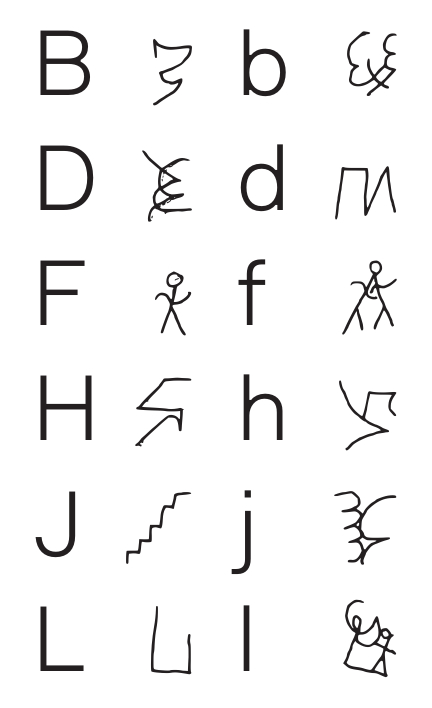
\includegraphics[width=80mm]{./img2.jpg}  
  %\hfill
%\end{adjustwidth}
  %\caption{Estátua equestre do general soviético Georgui Júkov (1896-1974), herói da resistência à invasão nazista, em frente ao Museu de História Russa, nas imediações da Praça Vermelha, em Moscou}

%\thispagestyle{empty}

%\end{figure}
%\end{vplace}

%\end{absolutelynopagebreak}